% SIAM Article Template
\documentclass[review,onefignum,onetabnum]{siamonline171218}

% Information that is shared between the article and the supplement
% (title and author information, macros, packages, etc.) goes into
% ex_shared.tex. If there is no supplement, this file can be included
% directly.
% SIAM Shared Information Template
% This is information that is shared between the main document and any
% supplement. If no supplement is required, then this information can
% be included directly in the main document.


% Packages and macros go here
\usepackage{lipsum}
\usepackage{amsfonts}
\usepackage{graphicx}
\usepackage{epstopdf}
\usepackage{algorithmic}

%usepackage[utf8]{inputenc}
\usepackage{textpos}
\usepackage{verbatim}
\usepackage{textcomp}
\usepackage{varwidth}
%\usepackage{graphicx}
%\usepackage{amsmath}
%\usepackage{amssymb}
%\usepackage{algorithmic}
%\usepackage[ruled]{algorithm2e}
%\usepackage[linesnumbered,ruled]{algorithm2e}
\ifpdf
  \DeclareGraphicsExtensions{.eps,.pdf,.png,.jpg}
\else
  \DeclareGraphicsExtensions{.eps}
\fi

% Prevent itemized lists from running into the left margin inside theorems and proofs
\usepackage{enumitem}
\setlist[enumerate]{leftmargin=.5in}
\setlist[itemize]{leftmargin=.5in}

% Add a serial/Oxford comma by default.
\newcommand{\creflastconjunction}{, and~}

% Used for creating new theorem and remark environments
\newsiamremark{remark}{Remark}
\newsiamremark{hypothesis}{Hypothesis}
\crefname{hypothesis}{Hypothesis}{Hypotheses}
\newsiamthm{claim}{Claim}

% Sets running headers as well as PDF title and authors
\headers{An adaptive Metropolis algorithm with rejection-based Gaussian proposal-scaling for fast convergence in multimodal parameter spaces}{Graham West, John Wallin}

% Title. If the supplement option is on, then "Supplementary Material"
% is automatically inserted before the title.
\title{An adaptive Metropolis algorithm with rejection-based Gaussian proposal-scaling for fast convergence in multimodal parameter spaces \thanks{Submitted to the editors DATE.
\funding{This work was funded by the Fog Research Institute under contract no.~FRI-454.}}}

% Authors: full names plus addresses.
\author{Graham West \thanks{Department of Computational Science, Middle Tennessee State University, Murfreesboro, TN 
  (\email{gtw2i@mtmail.mtsu.edu}).}
\and John Wallin \thanks{Department of Computational Science, Middle Tennessee State University, Murfreesboro, TN (\email{jwallin@mtsu.edu}).}}

\usepackage{amsopn}
\DeclareMathOperator{\diag}{diag}


%%% Local Variables: 
%%% mode:latex
%%% TeX-master: "ex_article"
%%% End: 


% Optional PDF information
\ifpdf
\hypersetup{
  pdftitle={An adaptive Metropolis algorithm with rejection-based Gaussian proposal-scaling for fast convergence in multimodal parameter spaces},
  pdfauthor={Graham West, John Wallin}
}
\fi

% The next statement enables references to information in the
% supplement. See the xr-hyperref package for details.
% SUPPLEMENT
% \externaldocument{ex_supplement}


% FundRef data to be entered by SIAM
%<funding-group>
%<award-group>
%<funding-source>
%<named-content content-type="funder-name"> 
%</named-content> 
%<named-content content-type="funder-identifier"> 
%</named-content>
%</funding-source>
%<award-id> </award-id>
%</award-group>
%</funding-group>

\begin{document}

%\setlength{\abovedisplayskip}{9pt}
%\setlength{\belowdisplayskip}{8pt}

\maketitle

% REQUIRED
\begin{abstract}
Performing MCMC parameter estimation on complex, nonlinear mathematical models can quickly lead to endless searching through highly multimodal parameter spaces. If one does not know the optimal proposal distribution, the burn-in period can take an excessively long time, due to the Markov chain not properly mixing and becoming trapped near a suboptimal mode. Also, if the model of interest is very computationally expensive, one would prefer to evaluate it as few times as possible. With these challenges in mind, we present in this paper an adaptive Metropolis method RSAP (rejection-scaled adaptive proposal) which can grow and shrink the scale of the Gaussian proposal width (independently for each parameter) based on the number of consecutive rejections the chain has encountered. The method is flexible and robust enough to handle parameter spaces that are both high-dimensional and multimodal (and correlated???). It also solves the issue of the unknown optimal proposal width by adjusting it over time. We will provide a proof of its ergodicity and conclude with comprehensive computational results implementing this method on a number of benchmark optimization functions, comparing its convergence to that of the standard Metropolis method.
\end{abstract}

% REQUIRED
\begin{keywords}
Markov chain Monte Carlo, adaptive methods, parameter estimation
\end{keywords}

% REQUIRED
\begin{AMS}
62M05 (markovian estimation), 62M09 (non-markovian estimation)
% 37, 49, 60, 63, 65, 68
% https://mathscinet.ams.org/msc/msc2010.html?t=62Mxx&btn=Current
\end{AMS}

\section{Introduction}
Markov chain Monte Carlo (MCMC) methods provide one of the most widely-used and easily accessible solution techniques to the problem of model parameter estimation (PE). As the name suggests, MCMC algorithms use Markov chains to sample the state space of the model being studied, thus obtaining distributions for all of its relevant parameters. With an ever-growing number of MCMC method types---from interacting forests of chains to delayed rejection techniques which approximate a full model evaluation---a suitable method can be found for virtually every problem.

This paper is outlined in the following way. First, we open with a review of the original Metropolis method, as well as some general notes on how kernel mixing and adaptive methods are able to increase its performance. Next, we will discuss our own adaptive kernel mixing method RSAP and the motivating factors for using it, as well as provide a proof of its ergodicity. Lastly, we will present and interpret results of experiments performed on our method using common optimization benchmark functions (including Gaussian, Rosenbrock, and Ackley functions) in several different dimensionalities, going into detail in comparing our method's performance with that of standard Metropolis over a range of proposal widths.


\subsection{Metropolis}
One of the most well-known and widely-used MCMC techniques is the original Metropolis method. First developed by Metropolis et al. \cite{Metro} and later generalized by Hastings \cite{Hastings}, this simple method has been the foundation for countless new and improved versions that have continued to build on the basic principles found within their predecessor.

Given data that we wish for the model to reproduce, the Metropolis method attempts to sample a distribution over the model parameters called the \textit{posterior}. This distribution will have a peak at the values of the model parameters which best approximate the data. However, we do not know the posterior since we cannot directly invert the parameter-data relationship (and since to do so would be to know the solution to the problem). Therefore, we must express it in terms of distributions which we do know. From Bayes theorem, we have
\begin{equation}
%	\pi(\theta|y) = \dfrac{\ell(y|\theta)p(\theta)}{p(y)} \propto \pi(y|\theta)p(\theta)
	\pi(\theta|y) \propto \ell(y|\theta)p(\theta)
\end{equation}
where $\pi$ is the \textit{posterior} distribution, $\ell$ is the \textit{likelihood} distribution, and $p$ is the \textit{prior} distribution. As opposed to the posterior---which tells us the probability of the model parameters given the data---the likelihood $\ell(y|\theta)$ tells us the probability of the data given the parameters. Therefore, we can easily calculate its value via a single model evaluation with the given parameters $\theta$ (referred to as the state). In addition, we may also have prior information about what parameter values are most likely to be realized in the actual system (for example, if the parameters can only take on values in a finite range or tend to be concentrated about a central mean). This information is incorporated via the prior distribution $p$. Together, the likelihood and prior help us to reconstruct the posterior distribution (up to a scale factor which does not impact the method) so that the inverse problem may be solved. 

Now, concerning the specifics of how the Metropolis method successfully samples the posterior, suppose we're given some data $y$ and an initial state $\theta_0$, which is a reasonable guess for the proper values of the parameters. The method generates new candidate states and pobabilistically accepts them based on their relative improvement from the current state, using the Bayesian approximation of the posterior as a metric. Candidate state generation is performed via sampling of the \textit{proposal} distribution $q(\theta_2|\theta_1)$, defined as the probability that a new state $\theta_2$ will be selected as a candidate for acceptance given the current state $\theta_1$. Whether acceptance or rejection is performed is determined by the \textit{acceptance probability} $\alpha(\theta_2|\theta_1)$, defined as the probability that the candidate state $\theta_2$ will be accepted given the current step $\theta_1$. Over time, the distribution created from the samples will conform to the posterior, at which point the method is said to have \textit{converged}. Below is a pseudocode implementation of Metropolis (Algorithm 1.1) which runs for $N$ steps.
% mention prior?
\begin{algorithm}[h]
\begin{algorithmic}[1]
	\STATE Initialize $\theta_0$
	\FOR{ $n = 1$ \TO $N$}
		\STATE Generate $\theta'_n \sim q(\theta'_n|\theta_{n-1})$
		\STATE \begin{varwidth}[t]{\linewidth}
		Compute $\alpha(\theta'_n|\theta_{n-1}) = \textrm{min}\Bigg(1, \dfrac{\pi(\theta'_n|y)} {\pi(\theta_{n-1}|y)}\Bigg)$ \par
		\hskip\algorithmicindent \hspace{1.20in} $=\textrm{min}\Bigg(1, \dfrac{\ell(y|\theta'_n)p(\theta'_n)} {\ell(y|\theta_{n-1})p(\theta_{n-1})}\Bigg)$
		\end{varwidth}
		\STATE Set $\theta_n = \theta'_n$ with probability $\alpha$, else $\theta_n = \theta_{n-1}$
	\ENDFOR
\end{algorithmic}
\caption{Metropolis-Hastings}
\end{algorithm}

%Steps 4-5 let the algorithm accept a new state with either better fitness than the previous state or only marginally less fitness. Several things are achieved by doing this. First, the majority of time is spent searching through regions of increasingly better fitness. Also, since worse solutions can still be accepted, the algorithm can still climb back out of false extrema.

Metropolis has several useful properties which contribute its great effectiveness. First---interpreting the method as an annealling-esque optimization method---it can both naively hill-climb and tactically accept poorer states to escape suboptimal local modes. When testing a new candidate state for acceptance, if it has an equal or higher posterior value than the current state, then $\alpha = 1$ and acceptance is guaranteed (hill-climbing). On the other hand, if the posterior is lower, then $1 > \alpha \ge 0$ and the poorer state still has a probability of being accepted. Though poorer states can be accepted, $\alpha$ decreases as the candidate's posterior becomes lower, so very poor candidates will usually be rejected. Counter-intuitively, this ability to accept poorer states is required to guarantee the eventual convergence of Metropolis (as evidenced by the appearance of the acceptance probability in the proof in the following paragraph).

This leads us to the second useful property of Metropolis. As long as the proposal distribution endows the Markov chain with a few key properties (irreducibility, aperiodicity, and non-transcience)---which hold for nearly all reasonable proposals---the distribution will always converge to the posterior, the stationary distribution of the chain formed by Metropolis. Assuming the three conditions mentioned above hold for the chain, we can easily show that the posterior distribution is the stationary distribution of the Metropolis method (proof taken from Gelman \cite{GelmanBayes}). Say the algorithm is at the $n$-th step and that $\theta_n = a$, where $a$ was drawn from the posterior. Now, suppose we propose the candidate $\theta_{n+1} = b$ such that $\pi(b) \ge \pi(a)$. Then,
\begin{equation}
		P(\theta_n = a, \theta_{n+1} = b) = \textrm{min}\Bigg(1, \dfrac{\pi(b)}{\pi(a)} \Bigg) q(b|a) \pi(a) = q(b|a) \pi(a)
\end{equation}
On the other hand, suppose $\theta_n = b$ and we attempt a transition to the candidate $\theta_{n+1} = a$. Then,
\begin{equation}
	\begin{split}
		P(\theta_n = b, \theta_{n+1} = a) & = \textrm{min}\Bigg(1, \dfrac{\pi(a)}{\pi(b)} \Bigg) q(a|b) \pi(b)
		\\
		& = \dfrac{\pi(a)}{\pi(b)} q(a|b) \pi(b) = q(a|b) \pi(a) = q(b|a) \pi(a)
	\end{split}
\end{equation}
Therefore, $P(\theta_n = a, \theta_{n+1} = b) = P(\theta_n = b, \theta_{n+1} = a)$, which is the condition for stationarity. 

Note that since the stationary distribution---being simply the posterior---is independent of the proposal used, and thus holds for all valid proposals. However, though the method is guaranteed to always converge to $\pi$, it may take a large number of steps for convergence to occur. Much of the algorithm's utility rests on the choice of a good proposal $q$. If one chooses too thin of a distribution, the method may have difficulty escaping suboptimal modes within an acceptable amount of time. On the other hand, too wide a distribution and the method might jump past true optimal modes or begin to oscillate about them, taking a large number of steps to sink into them.

With this in mind, the key question is, "What is the optimal proposal to use for problem $X$?" As should be expected, to know the answer to this question is essentially to know the solution to problem $X$. Therefore, certain assumptions and compromises must be made when designing proposals. Fortunately, as shall be seen in the following sections, this problem of the unknown proposal can be largely alleviated through clever means such as kernel mixing and adaptive proposals.

% use the words epistemic and ontic to refer to the different types of error

\subsection{Kernel mixing and composition}
Kernel mixing and composition are techniques where the transition probabilities (or kernel) used at each step in the chain may be different. Specifically, \textit{composition} refers to a method where the kernel is chosen at each step through some determinstic means. Consider, for example, the simple case we have two kernels $P_1, P_2$ and simply alternate between them, producing the $n$-step kernel $P_1P_2P_1P_2 \cdots P_k$, where $k = 1$ if $n$ is odd and $k = 2$ if $n$ is even (note that we use the convention commonly found in Markov chain literature of representing states as row vectors and right multiplying them by the kernel). 

On the other hand, techniques where the kernels used at each step are determined by some random process are termed \textit{mixing} methods. Consider another example where we have two kernels $P_1, P_2$, but instead of strictly alternating, we have a probability 0.5 of choosing either at any given step. Then, the kernel used at each step is simply $0.5 P_1 + 0.5 P_2$---the linear combination of the kernels and their respective probabilities---and the $n$-step kernel is $\big( 0.5 P_1 + 0.5 P_2 \big)^n$. Upon an actual run of this method, the true $n$-step kernel used is $P_{i_1} P_{i_2} \cdots P_{i_n}$ where the $i_j$ are determined by performing some random process on the given distribution. However, when run for a large number of steps, the second kernel will converge to the first. As shall be seen in section 2, our method uses kernel mixing by randomly selecting between numerous Gaussian proposals with varying widths.


\subsection{Adaptive MCMC}
% Significant MCMC researchers: Bedard, Rosenthal, Haario, Gelman, Roberts, Gilks

% adaptive proposal: scaling, covariance, learning search space

% Should we include general references like this from Haario AP in addition to citing specific algorithms or results: "The shape and the size of the proposal distribution q(.) is known to be very crucial for the convergence of the Markov chain corresponding the MCMC algorithm, see for example (Gelman, Roberts \& Gilks 1996), (Gilks, Richardson \& Spiegelhalter 1995), (Gilks, Roberts \& Sahu 1998) and (Roberts, Gelman \& Gilks 1994)."

Another technique for improving the performance of MCMC is to use so-called \textit{adaptive} methods which allow the kernel to intelligently adapt to the state space as more and more samples are obtained. The chains produced by these methods are referred to as \textit{inhomogeneous} chains since the kernel is not constant over time. For many models with nonlinear interactions between the parameters, neighboring regions in state space can have completely different posterior profiles, causing what would be an optimal proposal in one region to perform poorly in another. There may be numerous local modes clustered together or large plateaus. These effects combined with a lack of prior knowledge of which proposal should be chosen can inevitably lead to long run times. Thus, in these cases, one can justify the use of methods which can tune themselves based on the changing geometry of the state space.

Though adaptive methods can dramatically increase computational performance and efficiency, they often lose some of the desired analytical properties that their more simple counterparts have. For example, if the evolution of the kernel depends on the samples from multiple previous steps, the chain is no longer \textit{Markovian}. Also, in general, one cannot prove ergodicity without the assumption of several special conditions which may be difficult to verify in practice. Fortunately, even if one cannot verify convergence properties for a specific adaptive MCMC method, it may still be used to dramatically shorten the burn-in time as the chain searches for the target distribution. Despite the difficulties discussed, we were actually able to prove our own method's ergodicity through simple (yet notationally dense) means thanks to Theorem 5 from a paper by Roberts and Rosenthal \cite{RRAdaptErgo}. See this resource for a very thorough analysis on conditions for the convergence of adaptive MCMC methods.

% Also, since the proposal distribution is constantly changing scale, the transition probabilities are not \textit{stationary} either. This is not an issue, however, since most adaptive methods are meant to be used solely during burn-in time and then replaced by a method with more analytically desirable properties for remaining duration of the run.

% Also discuss Haario's adaptive proposal (AP)---which uses a fixed number of previous states---then AM---which uses all previous states and meets the diminishing adaptation criterion.

Two excellent examples of adaptive MCMC methods come from Haario, Saksman, and Tamminen in the form of the \textit{Adaptive Proposal} (AP) \cite{HaarioAP} and \textit{Adaptive Metropolis} (AM) \cite{HaarioAM} methods. While both methods are based on the same principle of adaptation, AM retains ergodicity while AP does not. The core principle shared by the two is the use of a continuously adapting Gaussian distribution as the proposal for the standard Metropolis method. Specifically, the proposal used is 
\begin{equation}
	q_n(\theta_2|\theta_1) = N(\theta_1, \bigg(\dfrac{2.38^2}{d}\bigg)\Sigma_n)
\end{equation}
where $\Sigma_n$ is the covariance matrix computed from samples generated over past steps. This allows the Gaussian to continually re-scale and re-orient itself as it encounters different regions of state space. Now, the only difference between AP and AM is that AP uses a fixed number of samples to calculate $\Sigma_n$ while AM uses the entire history of the chain. Thus, AP's adaptation does not vanish since its covariance matrix does not converge, while AM's does (due to the central limit theorem). 

\begin{comment}
From handbook:

"Another possibility (Roberts and Rosenthal, 2009) is to instead let the proposal be a
mixture distribution of the form:" $1 > \beta > 0$, must use only $\Sigma_0$ until $\Sigma_n$ is meaningful

\begin{equation}
	q_n(\theta_2|\theta_1) = (1-\beta) N(\theta_1, \bigg(\dfrac{2.38^2}{d}\bigg)\Sigma_n) + \beta N(\theta_1, \Sigma_0)
\end{equation}
\end{comment}

% One of the simplest ways to do so for the Metropolis method when using a Gaussian proposal distribution is to let the proposal's covariance matrix change as more samples are gathered (cite MCMC handbook). After a long run time, this covariance matrix should be approximately equal to the true covariance matrix associated with the model parameters. 

% As stated previously, most nonlinear problems have a search space which is highly multimodal, which can have a profound effect on an algorithm's burn-in time. In this situation, it is ideal to use a modified version of MH which allows the some aspect of the algorithm (say, the proposal distribution or the Hastings ratio) to change over time. Although standard MH is always guaranteed to converge eventually, this adaptive step can speed up the process dramatically.




%%%%%%%%%%%%%%%%%%
%%%%% BEGIN RSAP %%%%%%%
%%%%%%%%%%%%%%%%%%

\section{Rejection-scaled adaptive proposal (RSAP)}
We now move on to present our own contribution to the field of adaptive MCMC: the rejection-scaled adaptive proposal method (RSAP). Based on the original Metropolis method, this method uses very simple means to scale the entries of the Gaussian proposal's diagonal covariance matrix (i.e., the proposal widths in the direction of each model parameter) to more locally optimal values. We will begin with a discussion of our motivation for developing the method, the challenges it addresses, and some advantages it has over standard Metropolis and some other adaptive methods. We will then move on to a detailed description of the method on a step-by-step level and end with our ergodicity proof.


% 1D vs. ND, sigma vs. SIGMA
\subsection{Motivation and advantages}
% MCMC will always escape the mode, but will take forever sometimes. We speed it up.
There are two main advantages RSAP has over standard Metropolis or other adaptive methods. First, as we have discussed, it isn't possible in general to know a priori what the optimal proposal width should be for a given problem. Even if one chooses the optimal proposal width, this by no means guarantees that certain regions of state space might not be more efficiently traversed with a different proposal width. These issues are resolved by the ability of RSAP to both grow and shrink the proposal width at a set amplitude and rate, allowing the chain to escape local modes more easily and explore flatter regions more quickly.

% Therefore, we had to give the algorithm the ability to determine if it was not making progress---if, say, it were stuck in a false minimum---and alter the width of the Gaussian proposal (in each parameter's dimension separately) so that it might escape quicker than it would by simply waiting for an acceptable sample to be drawn from the original proposal.

Another advantage this method has over other more complicated adaptive methods is its trivial implementation and the minimal overhead it requires. Both the extra storage and computing time required for our method compared to standard Metropolis are negligible, since only several additional tuning parameters, counters, and scale factors must be stored and the adaptive scaling functions are computationally trivial to evaluate. Because of this, there is essentially no reason not to use RSAP as opposed to standard Metropolis.

\subsection{The method}
The key to the RSAP method is that it mixes a fixed-width Gaussian with two adaptable wide and thin Gaussians (one of each) into a single proposal. The thin option is included so that the chain can squeeze into tight optimal modes and the wide option so that the chain can both escape suboptimal modes and traverse state space quickly. The fixed option is included so that we always have a reasonable proposal to use in case the others adapt too much to be useful. With this reasoning in mind, the proposal for a single model parameter has the form of the linear combination
\begin{equation}
	q^n(\theta_{n+1}|\theta_n) = p_t^n N(\theta_n, \sigma_{t}^2) + p_f^n N(\theta_n, \sigma_{f}^2) + p_w^n N(\theta_n, \sigma_{w}^2)
%	q(\theta_2|\theta_1) = \dfrac{1}{3}N(\theta_1, \sigma_{thin}^2) + \dfrac{1}{3}N(\theta_1, \sigma_{fixed}^2) + \dfrac{1}{3}N(\theta_1, \sigma_{wide}^2)
\end{equation}
where $\sigma_{t} < \sigma_{f} < \sigma_{w}$. Every parameter uses separately adapting wide and thin proposal widths---allowing for independent adaptation of each---as well as its own fixed width (since the different parameters are likely different units/scales).

Concerning how we choose between the three options, we have the time-dependent probabilities $p_t^n, p_f^n, p_w^n$ that either the thin, fixed, or wide proposal (respectively) will be used. The following formulae govern the specific behavior of these probabilities.
\begin{equation}
	\begin{split}
		p_f^n & = \left\{
						\begin{array}{ll}
							1/3 & \quad 0 \leq n < n_1 \\
							2/3 - 1/3 \textrm{cos}( \pi (n - n_1)/n_2) & \quad n_1 \leq n < n_1 + n_2 \\
							1 & \quad n_1 + n_2 \leq n < N
						\end{array}
					\right.
		\\
		p_t^n = p_w^n & = (1 - p_f^n)/2
	\end{split}
\end{equation}
The intervals $n_1, n_2$ define three distinct regions for these functions. In the first region---which lasts $n_1$ steps---they describe a uniform distribution. In practice, $n_1$ should be set fairly large w.r.t. the total number of time steps so that RSAP has plenty of steps to utilize its adaptive features. The second region is a transition region---which lasts for $n_2$ steps---where proposal fixing begins to dominate the adaptation. From the definitions of $p_t^n, p_w^n$, there is an equal probability at each step that either thinning or widening will be chosen. There is no firm guideline for setting the second interval except $n_2 \leq N - n_1$, which is logically necessary. With the last region, we forced eventual convergence to $p_f^n \rightarrow 1$ as $n \rightarrow \infty$, and therefore ergodicity (see section 2.3).

Now, the values of $\sigma_{t}, \sigma_{w}$ adapt based on the number of recent consecutive rejections the chain has encountered, with their default values set to $\sigma_{f}$. If the candidate produced by the method is rejected, we choose from the three kernels based on the defined probability distribution. If the fixed kernel is chosen, then no adaptation is performed. However, if either the thin or wide kernels are used, then we increment one of the counters $k_{t}$, $k_{w}$ and compute the appropriate scale factor
\begin{equation}
	\begin{split}
		A_{t}(k_{t}) & = 1 - (1- \hat A_{t})(1-\textrm{exp}(-r_{t} k_{t}))\\
		A_{w}(k_{w}) & = 1 - (1- \hat A_{w})(1-\textrm{exp}(-r_{w} k_{w}))
	\end{split}
\end{equation}
where $r_{w}>0$, $r_{t}>0$, $\hat A_{w}>1$, and $1>\hat A_{t}>0$. (These functions---which are identical in form to the probability functions above---were chosen since their initial value is 1, their asymptotic limit is their respective $\hat A$ value, and their rate of convergence can be easily controlled via the $r$ constants.) We then set either $\sigma_{t} = A_{t} \sigma_{f}$ or $\sigma_{w} = A_{w} \sigma_{f}$ (depending on which was chosen) and perform a Metropolis step using this proposal width (again remembering that process is done independently for all parameters). On the other hand, whenever a candidate is accepted, the counters are reset to zero so that $\sigma_{t} = \sigma_{w} = \sigma_{f}$ (for all parameters).

To derive the full $M$-parameter proposal (which we do in section 2.3 with the help of a great deal of added notation), one has to consider all $3^M$ permutations of the $M$ parameters selecting the three different types of adaptation. It is helpful to do a two-parameter example. Each parameter will have its own set of proposal widths $\sigma_{t,m} < \sigma_{f,m} < \sigma_{w,m}$ ($m=1,2$). Upon adaptation, both parameters must choose which form of adaptation to apply, meaning there are $3^2$ possibilities for adaptation. Therefore, defining for the sake of notation $N(\theta_1, \sigma_1^2, \sigma_2^2)$ as a bivariate Gaussian distribution with diagonal covariance matrix given by the diagonal entries $(\sigma_1^2, \sigma_2^2)$, we can write the two-parameter proposal as
\begin{equation}
	\begin{split}
		q^n(\theta_{n+1}|\theta_n) = & \hspace{3pt} \sum_{i \in \{t,f,w\}} \sum_{j \in \{t,f,w\}} p_i^n p_j^n N(\theta_n,  \sigma_{i,1}^2, \sigma_{j,2}^2)
		\\
		= & \hspace{3pt} (p_t^n)^2 N(\theta_n, \sigma_{t,1}^2, \sigma_{t,2}^2) + p_t^n p_f^n N(\theta_n,  \sigma_{t,1}^2, \sigma_{f,2}^2) + p_t^n p_w^n N(\theta_n,  \sigma_{t,1}^2, \sigma_{w,2}^2) +
		\\
		& \hspace{3pt} p_f^n p_t^n N(\theta_n,  \sigma_{f,1}^2, \sigma_{t,2}^2) + (p_f^n)^2 N(\theta_n, \sigma_{f,1}^2, \sigma_{f,2}^2) + p_f^n p_w^n N(\theta_n,  \sigma_{f,1}^2, \sigma_{w,2}^2) +
		\\
		& \hspace{3pt} p_w^n p_t^n N(\theta_n, \sigma_{w,1}^2, \sigma_{t,2}^2) + p_w^n p_f^n N(\theta_n,  \sigma_{w,1}^2, \sigma_{f,2}^2) + (p_w^n)^2 N(\theta_n, \sigma_{w,1}^2, \sigma_{w,2}^2)
	\end{split}
\end{equation}

% mention the communication theory thing Hugh said, look up paper

% (being diagonal, it merely equalizes the proposal width for the different parameters since they might be different units and, thus, have different scales)


Algorithm 2.1 provides a pseudocode representation of the method.
\begin{algorithm}[h]
\algsetup{
	indent=12pt,
	linenosize=\small,
	linenodelimiter=.
}
\begin{algorithmic}[1]
	\STATE Initialize $\theta_0$, $\hat \Sigma$, $k_{w}^m = 0$, $k_{t}^m = 0$ for all $m=1, ..., M$
	
	\FOR{ $n = 1$ \TO $N$}
		\IF{ $n = 1$ \OR $\theta'_{n-1}$ was accepted}
			\STATE Set $\Sigma = \hat \Sigma$, $k_{w}^m = 0$, $k_{t}^m = 0$ for all $m$
		\ELSE
			\FOR{ $m = 1$ \TO $M$}
				\STATE Choose from \{wide, thin, fixed\} with probabilities \{$p_w^n, p_t^n, p_f^n$\}
%				\IF[increase]{0}
				\IF{wide}
					\STATE $k_{w}^m = k_{w}^m + 1$
					\STATE $A_{w}^m = 1 - (1-\hat A_{w})(1-\textrm{exp}(-r_{w} k_{w}^m))$
					\STATE $\Sigma_{mm} = A_{w}^m \hat \Sigma_{mm}$
%				\ELSIF[decrease]{1}
				\ELSIF{thin}
					\STATE $k_{t}^m = k_{t}^m + 1$
					\STATE $A_{t}^m = 1 - (1-\hat A_{t})(1-\textrm{exp}(-r_{t} k_{t}^m))$
					\STATE $\Sigma_{mm} = A_{thin}^m \hat \Sigma_{mm}$
%				\ELSE[initial]
				\ELSE
					\STATE $\Sigma_{mm} = \hat \Sigma_{mm}$
				\ENDIF
			\ENDFOR
		\ENDIF
		\STATE Generate $\theta'_n \sim N(\theta_{n-1},\Sigma)$
		\STATE Compute $\alpha(\theta'_n|\theta_{n-1}) =\textrm{min}\Bigg(1, \dfrac{\ell(y|\theta'_n)p(\theta'_n)} {\ell(y|\theta_{n-1})p(\theta_{n-1})}\Bigg)$
		\STATE Set $\theta_n = \theta'_n$ with probability $\alpha$, else $\theta_n = \theta_{n-1}$
	\ENDFOR
\end{algorithmic}
\caption{Rejection-scaled adaptive proposal (RSAP)}
\end{algorithm}We use a uniform prior over the given domain and a diagonal covariance matrix $\hat \Sigma$ for our fixed Gaussian. We define $N$ as the number of time steps and $M$ as the number of parameters. We also define separate counters $k_{w}^m$, $k_{t}^m$ and scale factors $A_{w}^m$, $A_{t}^m$ for every parameter $m = 1, ..., M$. As can clearly be seen, steps 3-20 are the additional adaptive functionality while steps 21-23 are from the standard Metropolis method.


\subsection{Ergodicty of RSAP}
x

CHANGES TO MAKE:

Consistent language, notation (hats) (RSAP, inhomogeneous MC)

talk about directionality on the graph



We will now provide some analysis of the method, proving conditions $a$ and $b$ of Theorem 5 from Roberts and Rosenthal \cite{RRAdaptErgo} for our method, thereby showing its ergodicity. Theorem 5 states that an adaptive method is ergodic if it is $a$) \textit{simultaneously uniformly ergodic} and has $b$) \textit{diminishing adaptation}. Condition $a$ means that all proposals which could be used in the adaptive method are themselves ergodic if used as proposals for standard Metropolis. Condition $b$ means that the "amount of adaptation" eventually vanishes, i.e., that the sequence of proposals converges (see \cite{RRAdaptErgo} for more rigorous definitions as well as a proof of Theorem 5). Condition $a$ clearly holds in the case of RSAP since the proposals are all Gaussians, which are ergodic. Therefore, the remainder of this section will be devoted to proving $b$.

\subsubsection{Proving diminishing adaptation}

Suppose there are $M$ parameters which RSAP must incorporate and that $\hat \Sigma$ is a fixed diagonal covariance matrix for these parameters. First, define the following as the \textit{elemental proposals}
\begin{equation}
	E((j_1,i_1), \cdots, (j_M, i_M)) = 	N(\theta_1, \Sigma)
\end{equation}
where
\begin{equation}
	\Sigma_{mm} = 
	\left\{
		\begin{array}{ll}
			\hat \Sigma_{mm} \cdot A_{t}(i_m) & \quad j_m = 1 \\
			\hat \Sigma_{mm} & \quad j_m = 2 \\
			\hat \Sigma_{mm} \cdot A_{w}(i_m) & \quad j_m = 3
		\end{array}
	\right.
\end{equation}
with their respective acceptance probabilities $a^n_{(j_1,i_1), \cdots, (j_M,i_M)} = \alpha(\theta'_{n+1}|\theta_n)$ where $m=1,...,M$ and $\theta'_{n+1}$ was drawn from the elemental proposal described by the subscripts. We let $n$ be the time step, the $i_m$'s be the adaptation degrees, and the $j_m$'s be switches that determine to which mode of adaptation the $i_m$'s are applied (1 = thin, 2 = fixed, 3 = wide). Note that $n$ and $i_m$ are non-negative integers such that $n \ge i_m$ since, in practice, the degree of adaptation cannot exceed the number of time steps which have occured. For the sake of space limitations in this paper, we will also define the rejection probability $r^n_{(j_1,i_1), \cdots, (j_M,i_M)} = 1- a^n_{(j_1,i_1), \cdots, (j_M,i_M)}$.

Next, define the following linear combinations as the \textit{adaptive proposals}
\begin{equation}
	q^n_{i^1_1, i^2_1, i^3_1, \cdots, i^1_M, i^2_M, i^3_M} = \bigg( \sum^{3}_{j_1=1} p_{j_1}^n \cdots \sum^{3}_{j_M=1} p_{j_M}^n E((j_1,i^{j_1}_1), \cdots, (j_M, i^{j_M}_M)) \bigg)
\end{equation}
with their associated acceptance probabilities
\begin{equation}
	b^n_{i^1_1, i^2_1, i^3_1, \cdots, i^1_M, i^2_M, i^3_M} = \bigg( \sum^{3}_{j_1=1} p_{j_1}^n \cdots \sum^{3}_{j_M=1} p_{j_M}^n a^n_{(j_1,i^{j_1}_1), \cdots, (j_M, i^{j_M}_M)} \bigg)
\end{equation}
%for all $n = \sum_{j = 1}^{3} i^j_m$.
This is the $M$-parameter generalization of the one- and two-parameter proposals from section 2.2 with the subscripts $t,f,w$ replaced with $1,2,3$, respectively. Let's examine Equation 2.5 more closely before continuing on. Regarding the indices, the integers $i^1_m$ are the degrees of proposal-\textit{thinning} adaptation while the integers $i^3_m$ are the degrees of proposal-\textit{widening} adaptation. The integers $i^2_m$ can be thought of as the degrees of proposal-\textit{fixing} adaptation (clearly a meaningless notion). They are merely auxiliary indices which help to establish conservation of adaptation degrees. Regarding the sums, there is one per parameter and their indices cover the three adaptation options so that the probability of choosing the elemental proposal $E((j_1,i^{j_1}_1), \cdots, (j_M, i^{j_M}_M))$ is $p_{j_1}^n \cdots p_{j_M}^n$.

\begin{comment}
A helpful (though not exactly correct) way to think about the generalization from $\hat q$ to $q'$ is to think of $q'$ as an $M$-fold direct product of $\hat q$ with itself. Abusing notation momentarily, define $E((s_1,k_1)) \times E((s_2, k_2)) = E((s_1,k_1), (s_2, k_2))$. Then, $q'$ can be written
\begin{equation}
	q'_{i^1_1, i^2_1, i^3_1, \cdots, i^1_M, i^2_M, i^3_M} =  \prod_{m=1}^{M} \dfrac{1}{3} \bigg( E((1,i^{1}_m)) + E((2,i^{2}_m)) + E((3,i^{3}_m)) \bigg)
\end{equation}
(This equation is written for purely instructive purposes, and is not utilized in any way in the proof or the algorithm itself.)
\end{comment}

Lastly, define $Q^n$ as the \textit{full proposal} at time-step $n$. Since acceptance and rejection are random phenomena, we cannot know ahead of time which specific elemental or adaptive proposal will be used at time step $n$. Thus, the full proposal will be a linear combination of the adaptive proposals whose total adaptation degrees are less than or equal to $n$ (since there could only have been up to $n$ rejections and, therefore, $n$ adaptations) with functions of their respective acceptance probabilities.

Let us now examine the structure of the full proposal and how it evolves throughout a run, temporarily restricting ourselves to one dimension for simplicity. Below, Figure 1 prodives a graphical representation of the flow of proposals during a run.
\begin{figure}[!h]
	\centering
	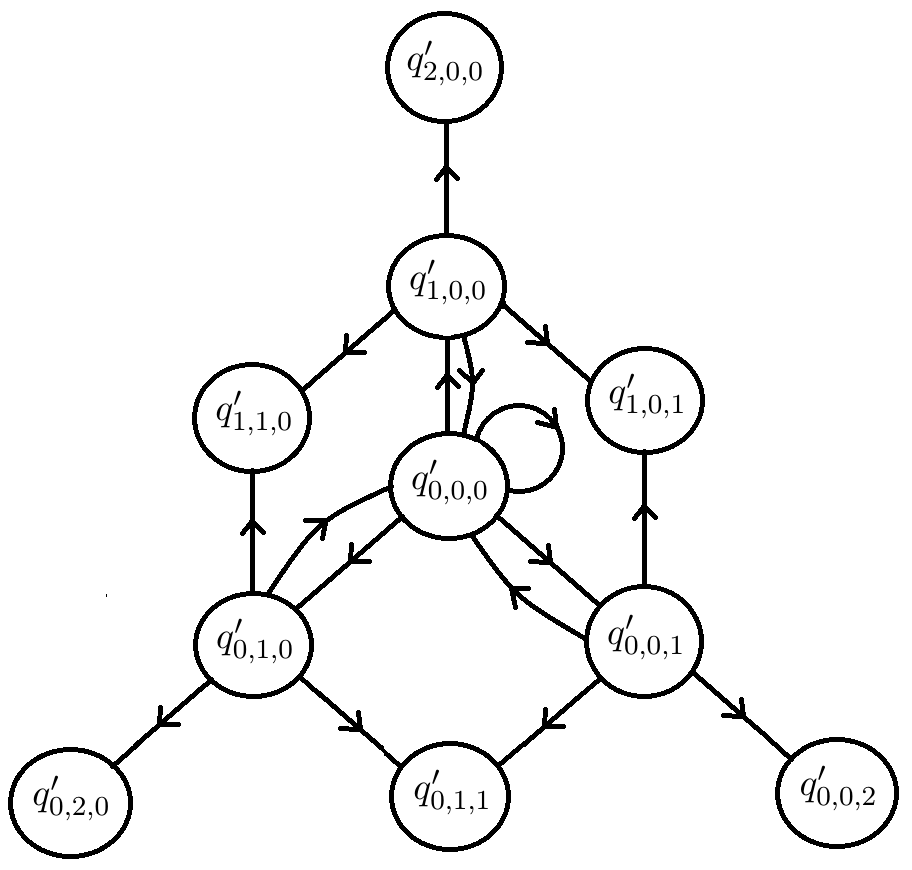
\includegraphics[scale = 0.3]{RSAP_True_02}
%	\vspace{-40pt}
	\caption{A graphical depiction of the method and the possible transitions that can take place from step one to two. At any state in the graph, four transitions can occur: increasing one of the three indices (rejection) or returning to the initial state.}
\end{figure}
One can think of method runs as paths through this graph. The first state is always $q'_{0,0,0}$ since no adaptation has yet taken place. Consequently, the first full proposal $q^0$ is also $q'_{0,0,0}$. As illustrated by the graph, there are four possible transitions from any given state (transitions back to $q'_{0,0,0}$ not shown). If acceptance occurs, the state returns to $q'_{0,0,0}$ (the fixed proposal with no adaptation). Alternatively, if the candidate is rejected, we will increment the adaptive degree indices corresponding to the elemental proposal which was used. For example, suppose that we chose to use a thin elemental proposal and the sample drawn from it was rejected. Then, we increment the thin proposal index so that the adaptive proposal used in the next time step will be $q'_{1,0,0}$. We can represent this mathematically with linear combinations of the adaptive proposals. Equations 2.8 below show the full proposals through $q^2$.
\begin{equation}
	\begin{split}
		Q^0 = & \hspace{3pt} q_{0,0,0}^0
		\\
		Q^1 = & \hspace{3pt} b^0_{0,0,0} q_{0,0,0}^1 + r^0_{(1,0)} p^0_1 q_{1,0,0}^1 + r^0_{(2,0)} p^0_2 q_{0,1,0}^1 + r^0_{(3,0)} p^0_3 q_{0,0,1}^1
		\\
		Q^2 = & \hspace{3pt} \Big( b^1_{0,0,0} b^0_{0,0,0} + b^1_{1,0,0} r^0_{(1,0)} p^0_1 + b^1_{0,1,0} r^0_{(2,0)} p^0_2 + b^1_{0,0,1} r^0_{(3,0)} p^0_3 \Big) q_{0,0,0}^2 + 
		\\
		& \hspace{3pt} r^1_{(1,0)} p^1_1 b^0_{0,0,0} q_{1,0,0}^2 + r^1_{(2,0)} p^1_2 b^0_{0,0,0} q_{0,1,0}^2 + r^1_{(3,0)} p^1_3 b^0_{0,0,0} q_{0,0,1}^2 +
		\\
		& \hspace{3pt} r^1_{(1,1)} p^1_1 r^0_{(1,0)} p^0_1 q_{2,0,0}^2 + r^1_{(2,1)} p^1_2 r^0_{(1,0)} p^0_1 q_{1,1,0}^2 + r^1_{(3,1)} p^1_3 r^0_{(1,0)} p^0_1 q_{1,0,1}^2 +
		\\
		& \hspace{3pt} r^1_{(1,1)} p^1_1 r^0_{(2,0)} p^0_2 q_{1,1,0}^2 + r^1_{(2,1)} p^1_2 r^0_{(2,0)} p^0_2 q_{0,2,0}^2 + r^1_{(3,1)} p^1_3 r^0_{(2,0)} p^0_2 q_{0,1,1}^2 +
		\\
		& \hspace{3pt} r^1_{(1,1)} p^1_1 r^0_{(3,0)} p^0_3 q_{1,0,1}^2 + r^1_{(2,1)} p^1_2 r^0_{(3,0)} p^0_3 q_{0,1,1}^2 + r^1_{(3,1)} p^1_3 r^0_{(3,0)} p^0_3 q_{0,0,2}^2
	\end{split}
\end{equation}
As can be seen (and was mentioned earlier), $Q^n$ contains all adaptive proposals of total degree up to $n$, i.e., $i_1^1+i_1^2+i_1^3 \le n$ (for $M$ parameters, this inequality holds for all parameters simultaneously) . We can write $Q^n$ succinctly as
\begin{equation}
	Q^n = \sum^n_{\ell=0} \Bigg(\sum_{i_1^1+i_1^2+i_1^3=\ell} c^n_{i_1^1,i_1^2,i_1^3} q_{i_1^1,i_1^2,i_1^3}^n \Bigg)
\end{equation}
where
\begin{align}
	\sum^n_{\ell=0} \Bigg(\sum_{i_1^1+i_1^2+i_1^3=\ell} c^n_{i_1^1,i_1^2,i_1^3} \Bigg) = 1
\end{align}
defines our normalization (since some proposal must always be chosen) and the inner sums are taken over all possible values of the three indices such that their sum is less than or equal to $n$. The value $c^n_{i_1^1,i_1^2,i_1^3}$ can be interpreted as the probability that that the adaptive proposal defined by the subscripts will be used at step $n$.

Now, returning to $M$ parameters, let us generalize the above formulae. The full proposal is written
\begin{equation}
	Q^n = \sum^n_{\ell=0} \Bigg(\sum_{i^1_m+i^2_m+i^3_m=\ell} c^n_{i^1_1, i^2_1, i^3_1, \cdots, i^1_M, i^2_M, i^3_M} q_{i^1_1, i^2_1, i^3_1, \cdots, i^1_M, i^2_M, i^3_M}^n \Bigg)
\end{equation}
with normalization
\begin{align}
	\sum^n_{\ell=0} \Bigg(\sum_{i^1_m+i^2_m+i^3_m=\ell} c^n_{i^1_1, i^2_1, i^3_1, \cdots, i^1_M, i^2_M, i^3_M} \Bigg) = 1
\end{align}
where $m = 1, \cdots, M$. We can construct several recurrence relations which describe how the values of the coefficients $c^n$ change over time. We get one relation which governs the evolution of the coefficient corresponding to the proposal which has zero total adaptation degree and another which governs all the rest.
\begin{equation}
	\begin{split}
		c^{n+1}_{0,0,0, \cdots, 0,0,0} = & \hspace{3pt} \sum^n_{\ell=0} \Bigg(\sum_{i^1_m+i^2_m+i^3_m=\ell} b^n_{i^1_1, i^2_1, i^3_1, \cdots, i^1_M, i^2_M, i^3_M} c^n_{i^1_1, i^2_1, i^3_1, \cdots, i^1_M, i^2_M, i^3_M}
		\\
		c^{n+1}_{i^1_1, i^2_1, i^3_1, \cdots, i^1_M, i^2_M, i^3_M} = & \hspace{3pt} \sum_{j_1 \mid i^{j_1}_1 \ge 1} \cdots \sum_{j_M \mid i^{j_M}_M \ge 1} \Big( r^n_{(j_1,i^{j_1}_1), \cdots, (j_M,i^{j_M}_M)} \Big) \Big( p^n_{j_1} \cdots p^n_{j_M} \Big) \cdot
		\\
		& \hspace{3pt} c^{n}_{i^1_1, \cdots, i^{j_1}_1-1, \cdots, i^3_1, \cdots, i^1_M, \cdots, i^{j_M}_M-1, \cdots, i^3_M}
	\end{split}
\end{equation}
The first relation is fairly basic, as it simply was derived from the fact that the adaptation-less proposal will be used at any step which immediately follows an acceptance. Consequently, it finds the total, weighted probability of acceptance given all possible proposals which could be used at that step. This is equal to the probability that the adaptation-less proposal will be chosen at the following step. The second relation is more complicated. From a top level perspective, it finds the total, weighted inflowing probability from all proposals which could possibly precede the proposal under consideration. More specifically, it does this by summing the rejection probabilities over all valid permutations of subtracting one from the three types adaptation degrees for all $M$ parameters (of which there are no more than $3^M$ permutations). By valid, we mean that subtracting one does not give a negative adaptation degree (thus the $\ge 1$ under the sums).

% is it confusing which time step is being referred to as current/previous?

Now, to prove diminishing adaptation, we will show that the values of $c^{n}_{i^1_1, i^2_1, i^3_1, \cdots, i^1_M, i^2_M, i^3_M}$ will vanish as $n \rightarrow \infty$ for any proposals that have at least one degree of either thinning or widening adaptation in at least one parameter. We will use induction on the thinning and widening adaptation degrees to prove this.

Let us first prove the base case, where we consider a proposal such that each parameter has only one adaptation degree assigned and there exists at least parameter such that its mode of adaptation is either thinning or widening. Without loss of generality, we will say that this is the first parameter and that thinning was chosen (the widening case is identical). Letting $c^{n}_{1, 0, 0, \cdots, j^1_M, j^2_M, j^3_M}$ be the coefficient of this proposal, this implies that either $j^1_m=1$ or $j_m^3=1$ for every $m = 2, \cdots, M$. Then, using the recurrence relation, we get
\begin{equation}
	c^{n+1}_{1, 0, 0, \cdots, j^1_M, j^2_M, j^3_M} = \Big( r^n_{(1,0), \cdots, (j_M,i^{j_M}_M)} \Big) \Big( p^n_{1} \cdots p^n_{j_M} \Big) \Big( c^{n}_{0,0,0, \cdots, 0,0,0} \Big)
\end{equation}
Now, all the terms in ths equation are bounded between 0 and 1 and $p_1^n \rightarrow 0$ as $n \rightarrow \infty$. Therefore, $c^{n+1}_{1, 0, 0, \cdots, j^1_M, j^2_M, j^3_M} \rightarrow 0$, as well, and we have that all coefficients with at least one parameter having a single adaptive degree assigned to either thinning or widening vanish.

We will now prove the induction step, which states that if any coefficient with at least one parameter having at least one thinning or widening adaptive degree vanishes, then the coefficients for all proposals that it precedes by one time step (in the sense of the discussion of Equation 2.14) do as well. Consider $c^{n}_{i^1_1, i^2_1, i^3_1, \cdots, i^1_M, i^2_M, i^3_M}$, which has at least one parameter with at least one thinning or widening adaptive degree. Equation 2.14 applied to this coefficient contains the coefficients for all possible preceding states. Now, since there is at least one degree of thinning or widening adaptation in the coefficient under consideration, every term in the sum from Equation 2.14 can be classified in one of two ways: either 1) that adaptation degree was obtained from the immediately preceding step or 2) from an earlier step. If it is from the immediately preceding step, we can factor out the appropriate probability term as we did for the base case, causing that term to vanish. If it was from an earlier step, then the proposal associated with that term already has at least one parameter with at least one thinning or widening adaptive degree, and thus---according to the induction hypothesis---vanishes. Having shown that every term in the sum vanishes, we have shown that all proposal coefficients with at least one parameter with at least one thinning or widening adaptive degree also vanish. Thus, the only non-vanishing coefficients are those for purely fixing proposals, which are all identical to the adaptation-less proposal. Therefore, the full proposal $Q^n \rightarrow q^{n}_{0,0,0, \cdots, 0,0,0}$ as $n \rightarrow \infty$, and we have diminishing adaptation, thus proving the ergodicity of RSAP.


\section{Computational testing}
Having proven the analytical integrity of our method, we now move on to demonstrate its practical utility through the presentation of numerous computational results. These cover multiple different aspects of the method's performance, including flexibility/robustness, mixing efficiency, and rate of convergence. We also present results from a new optimization-style test we developed in which we find the cumulative probability distribution for convergence of the chain to the global minimum of the test function, versus both an interval of initial states (1D only) and a range of fixed proposal widths (1D-MD???). This technique provides easy-to-interpret results which are numerically \textit{and} visually simple to compare.


\subsection{Discussion of RSAP parameters values used in testing}
When performing numerical experiments on our method, we used standard optimization test functions (including Gaussians, Rosenbrock functions, and Ackley functions), each with a global minimum of $y = f(\theta^*) = 0$ (with the exception of the bi-modal function). As such, the likelihood function can be expressed as
\begin{equation}
	\begin{split}
		\ell(y|\theta) & \propto \textrm{exp}(-\dfrac{1}{2} \dfrac{(y-(f(\theta)+\epsilon))^2}{\Delta^2})\\
					& \propto \textrm{exp}(-\dfrac{1}{2} \dfrac{(f(\theta)+\epsilon)^2}{\Delta^2})\\
	\end{split}
\end{equation}
where $\epsilon$ is an error term which we include in some of the tests below. The value of $\Delta$ affects the ease of acceptance, and thus the relative peakedness of the resulting sample-binned approximation of the posterior. Not knowing its proper value, we include it as a parameter for RSAP to estimate, though we set its proposal width quite low so that it does not change too rapidly, dramatically altering the acceptance rate.

There is also the matter of setting the adaptation parameters to their proper values. Clearly, the optimal values of these parameters are problem-dependent; so we attempted to find a set of reasonable values which improved the performance gain over Metropolis for as many test cases as possible. We thus arrived at maximum scaling magnitudes of $\hat A_{t} = 0.1, \hat A_{w} = 10$, respectively. Being able to both increase and decrease the propsal width by an order of magnitude ensures that the true optimal width is likely contained within the interval $[\hat A_t \sigma_f, \hat A_w \sigma_f]$. Next, concerning the scaling rates, we found that their values were less significant than the magnitudes in determining performance gain. Their values were set to $r_{t} = r_{w} = 0.3$, since this puts the scaling to within approximately 5\% of its maximum effect within 10 rejection steps ($e^{-0.3 \cdot 10} \approx 0.049$). Any longer would take too long to reach maximum scaling and frequent acceptances would leave the more extreme scaling values unused. Lastly, the probability scaling intervals $n_1, n_2$ are likely the most problem-dependent parameters since they determine how long RSAP is allowed to be adaptive. As discussed earlier, $n_1 < N$ should be large w.r.t. $N$ while $n_2 \leq N - n_1$ has more freedom. Because of their problem dependence, we will vary them throughout the tests.

WHY did we use these test functions? Cite Ackley, Rosenbrock, others. Justify usage.

INCLUDE results of modifying adaptation parameters???

UPDATE RSAP Workflow

REDO trace plots and things


\subsection{Chain mixing}
x

https://python-graph-gallery.com/111-custom-correlogram/

To begin our analysis, we will provide trace plots of one-parameter chains created by RSAP for the test functions under consideration, as well as plots of the functions used and sample-binned approximations of the posterior distribution. We will start with the 1D Gaussian defined by
\begin{equation}
	f(x) = a \Big( 1 - \textrm{exp}(-\dfrac{1}{2} \dfrac{x^2}{b^2}) \Big)
\end{equation}
where $a = 1, b = 0.3, x \in [-1, 1]$. The initial state values were set to $x_0 = 0.8, \Delta_0 = 0.08$ and the fixed proposal widths were set to $\sigma_x = 0.1, \sigma_\Delta = 0.0008$. As discussed above, the parameters for RSAP were set to $\hat A_{t} = 0.1, \hat A_{w} = 10, r_{t} = 0.3, r_{w} = 0.3, n_1 = 2000, n_2 = 1000$.
\begin{figure}[!htb]
\minipage{0.33\textwidth}
	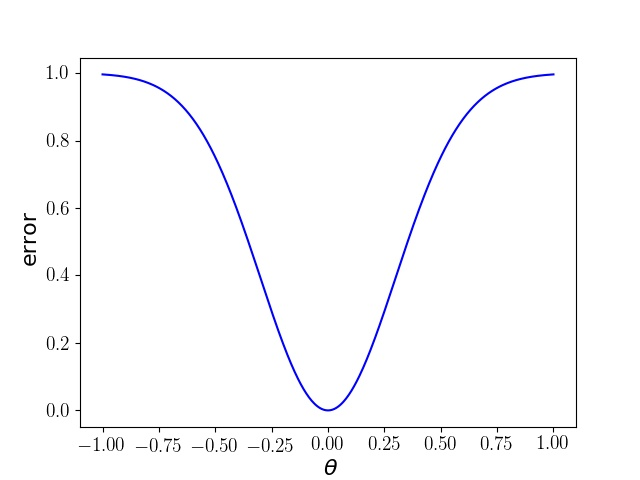
\includegraphics[width=\linewidth]{UQPlot_Gaussian_00_Function.jpg}
\endminipage\hfill
\minipage{0.33\textwidth}
	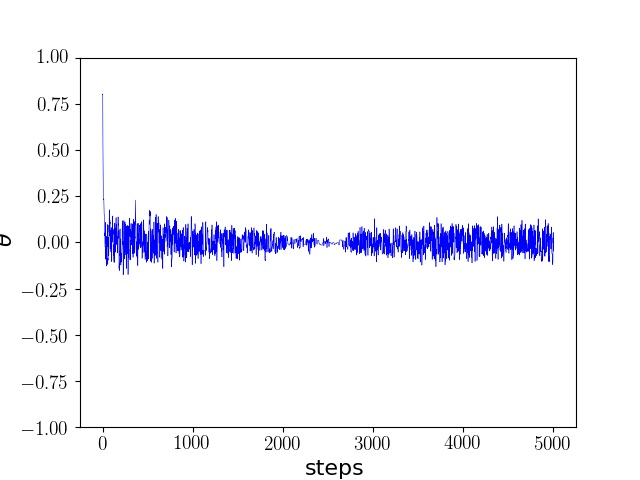
\includegraphics[width=\linewidth]{UQPlot_Gaussian_00_Trace.jpg}
\endminipage\hfill
\minipage{0.33\textwidth}%
	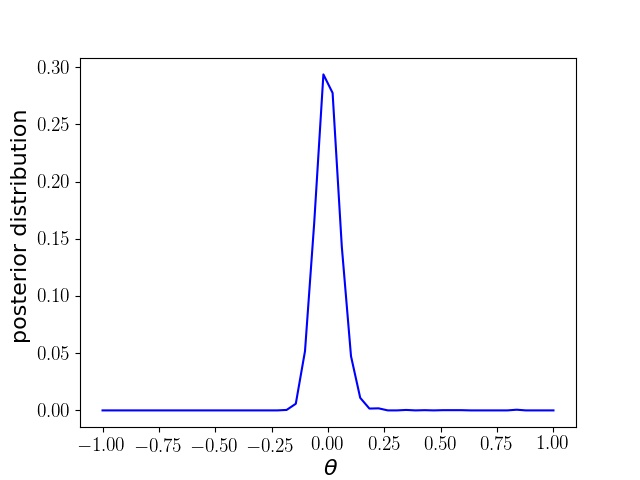
\includegraphics[width=\linewidth]{UQPlot_Gaussian_00_Posterior.jpg}
\endminipage
\caption{Plots of the Gaussian function, chain trace, and binned posterior estimate resulting from a run with 5,000 steps. In the trace plot in the center, the blue curve is the actual chain and red curve contains the only points with the highest posterior values up to the current time step. For the posterior plot on the right, we used 45 bins to get the image for the posterior distribution.}
\end{figure}
The Gaussian is such a simple function that there is no need to use adaptation on it, but it is a good control nonetheless.

Next, we have an Ackley function in 1D defined by
\begin{equation}
	f(x) = a \Big( 1 - \textrm{exp}(- 0.2 \sqrt{x^2/c}) \Big) + b \Big( e - \textrm{exp}(\textrm{cos}(2 \pi x)/c) \Big)
\end{equation}
where $a = 20, b = 4, c = 1, x \in [-10, 10]$. The initial state values were set to $x_0 = 8, \Delta_0 = 3.5$ and the fixed proposal widths were set to $\sigma_x = 1.0, \sigma_\Delta = 0.01$. The RSAP parameters again were set to $\hat A_{t} = 0.1, \hat A_{w} = 10, r_{t} = 0.3, r_{w} = 0.3, n_1 = 2000, n_2 = 1000$.
\begin{figure}[!htb]
\minipage{0.33\textwidth}
	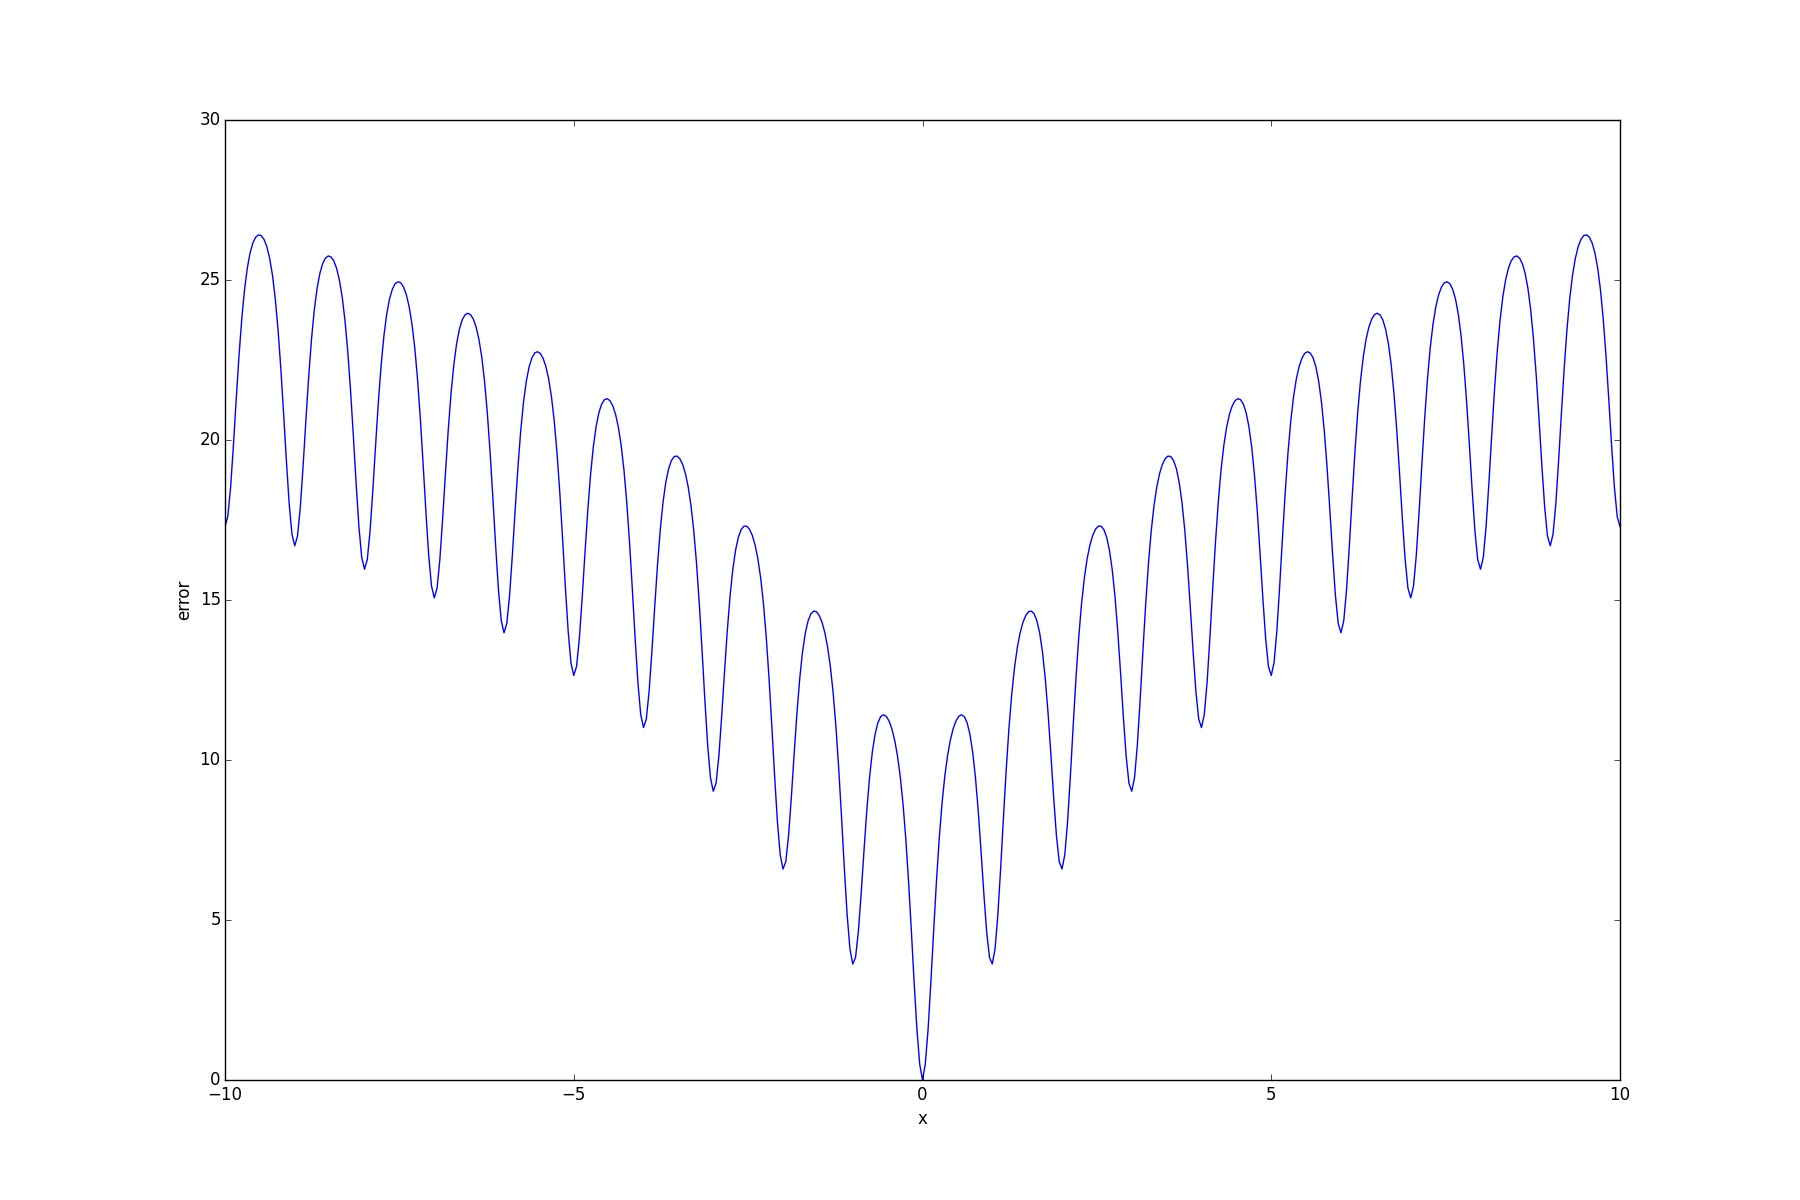
\includegraphics[width=\linewidth]{UQPlot_Ackley_00_Function.jpg}
\endminipage\hfill
\minipage{0.33\textwidth}
	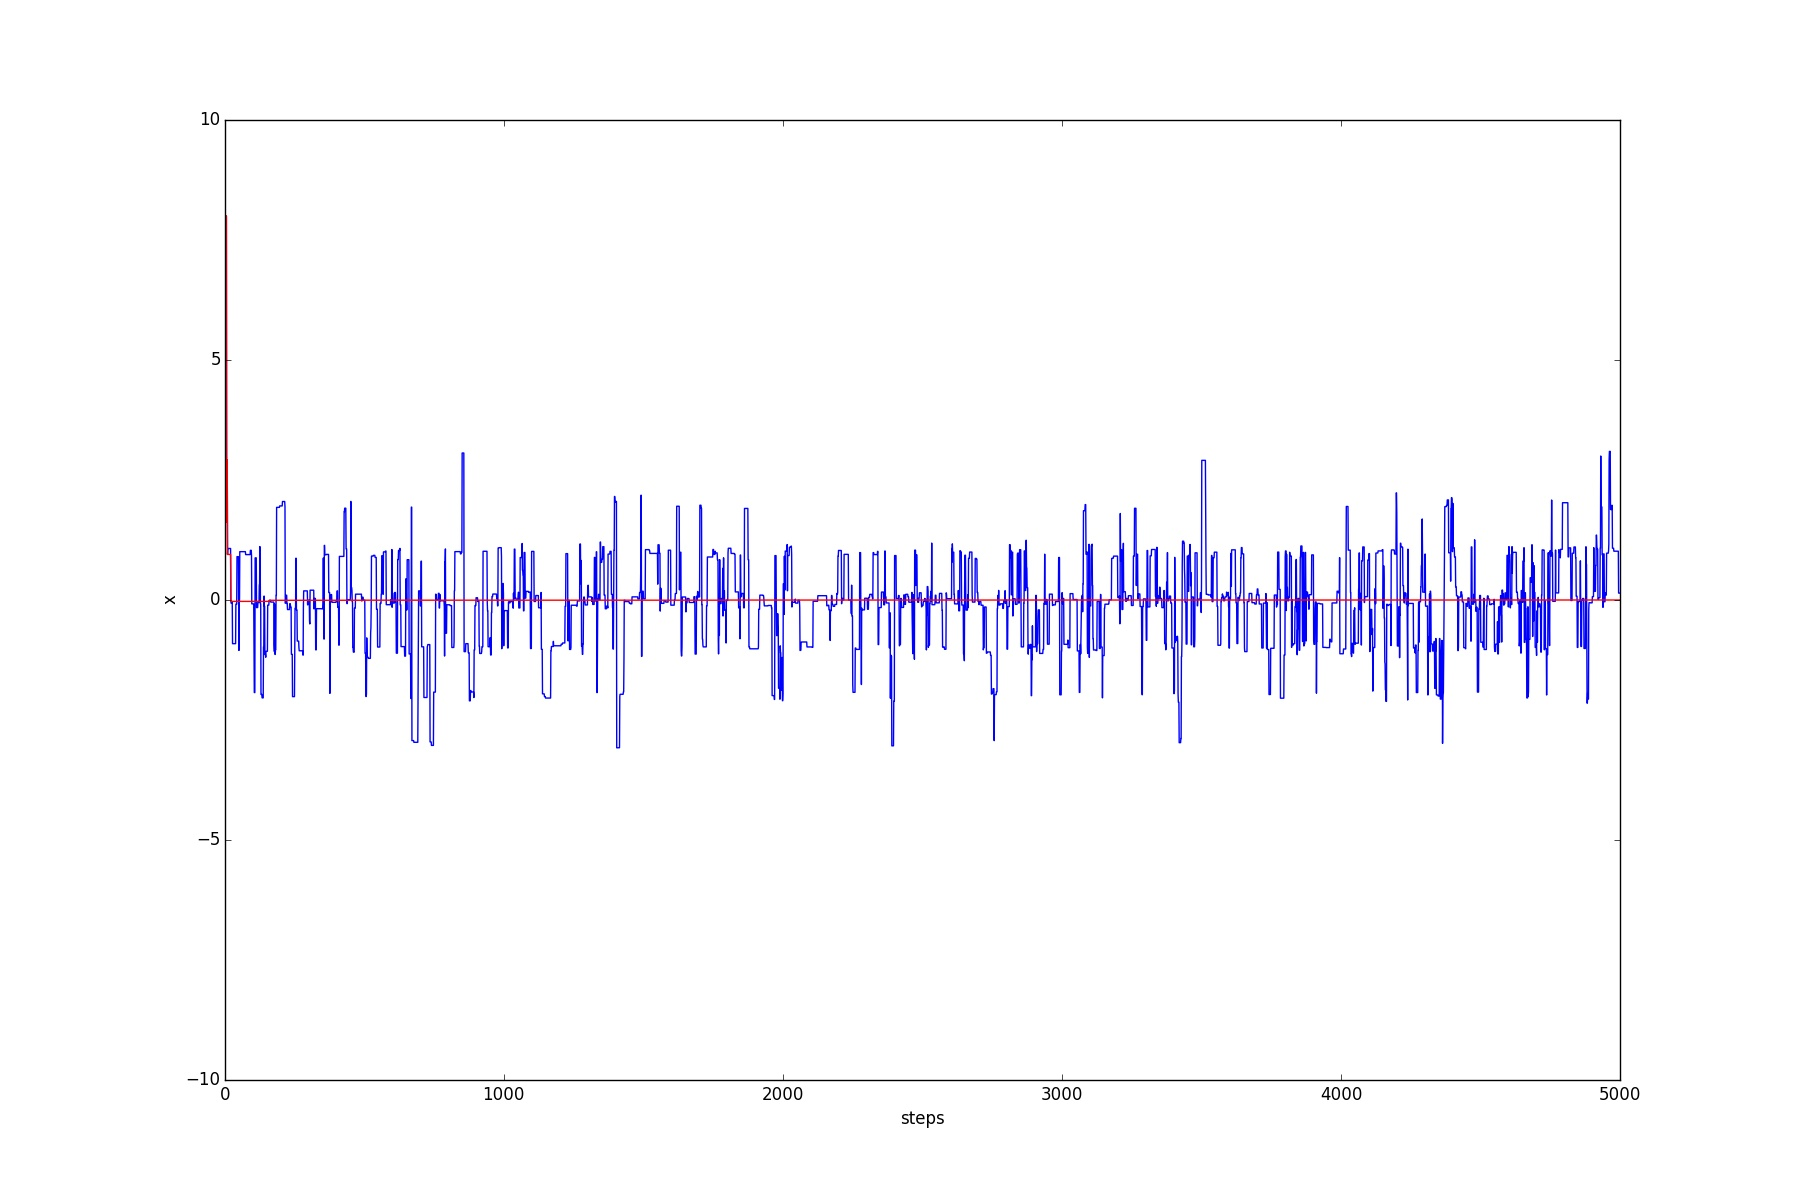
\includegraphics[width=\linewidth]{UQPlot_Ackley_00_Trace.jpg}
\endminipage\hfill
\minipage{0.33\textwidth}
	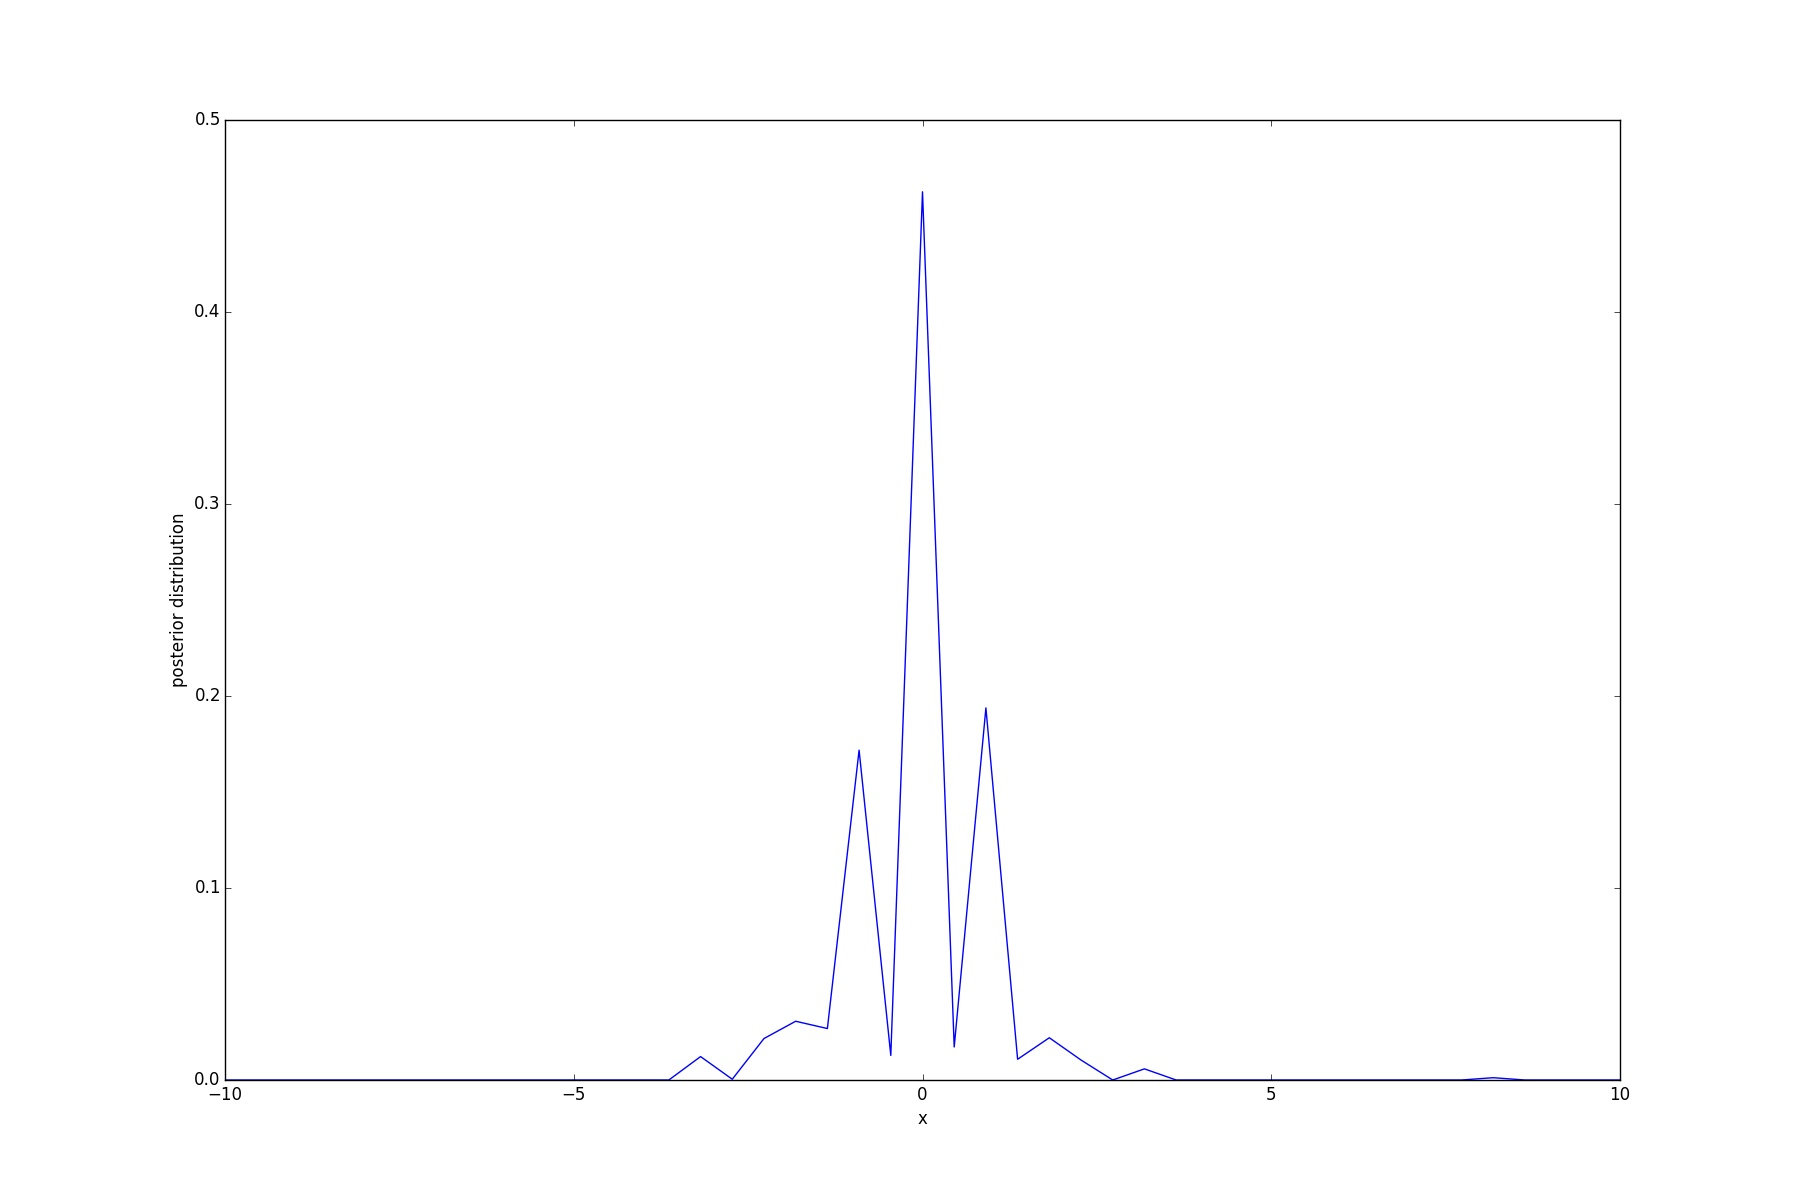
\includegraphics[width=\linewidth]{UQPlot_Ackley_00_Posterior.jpg}
\endminipage
\caption{Plots of an Ackley function, chain trace, and binned posterior estimate resulting from a run with 5,000 steps.}
\end{figure}
It is very easy to see from the trace and posterior plots that RSAP efficiently samples the modes near the center.

Lastly, we have a rather illustrative example of the superiority of RSAP to standard Metropolis in the form of a bi-modal function defined by
\begin{equation}
	f(x) = a \Big( 1 - \textrm{exp}(-\dfrac{1}{2} \Big( \dfrac{(x-c)^2}{b^2} \Big)^{d/2} ) \Big) + a \Big( 1 - \textrm{exp}(-\dfrac{1}{2} \Big( \dfrac{(x+c)^2}{b^2} \Big)^{d/2} ) \Big)
\end{equation}
where $a = 0.5, b = 0.333, c = 0.15, d = 8, x \in [-1, 1]$. The initial state values were set to $x_0 = 0.8, \Delta_0 = 0.08$ and the fixed proposal widths were set to $\sigma_x = 0.1, \sigma_\Delta = 0.0008$. As discussed above, the parameters for RSAP were set to $\hat A_{t} = 0.1, \hat A_{w} = 10, r_{t} = 0.3, r_{w} = 0.3, n_1 = 2000, n_2 = 1000$.
\begin{figure}[!htb]
\minipage{0.33\textwidth}
	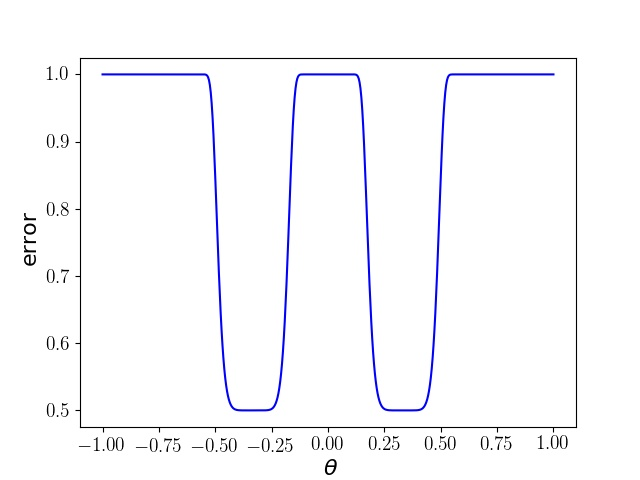
\includegraphics[width=\linewidth]{UQPlot_Bimodal_00_Function.jpg}
\endminipage\hfill
\minipage{0.33\textwidth}
	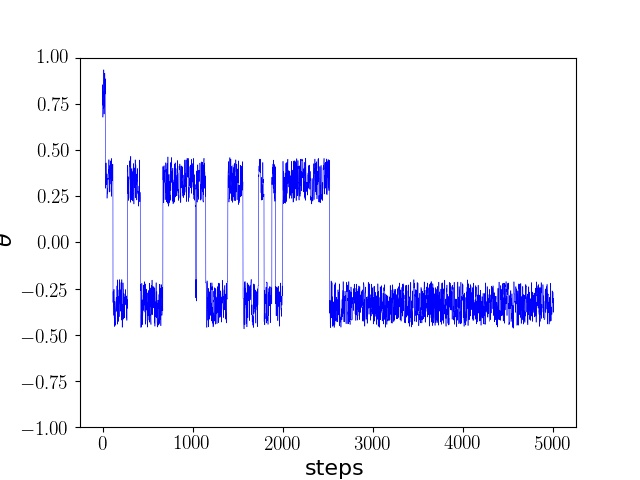
\includegraphics[width=\linewidth]{UQPlot_Bimodal_00_Trace.jpg}
\endminipage\hfill
\minipage{0.33\textwidth}
	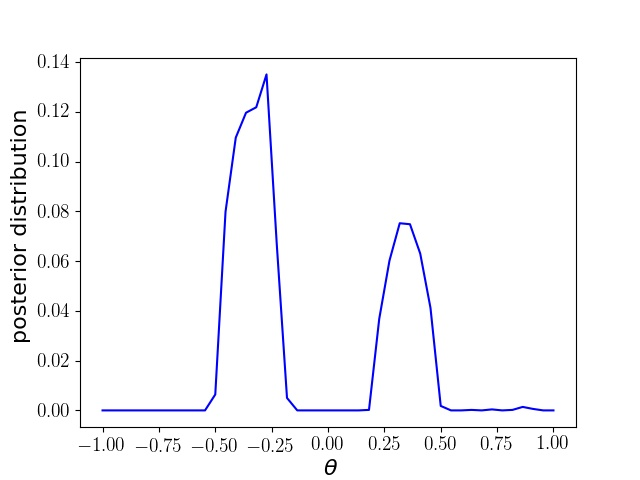
\includegraphics[width=\linewidth]{UQPlot_Bimodal_00_Posterior.jpg}
\endminipage
\caption{Plots of the bimodal function, chain trace, and binned posterior estimate resulting from an RSAP run with 5,000 steps.}
\end{figure}
As can be seen, there is efficient mixing between the two modes in the region up until $n = n_1$. Once standard Metropolis begins to overtake the adaptive effects, the chain becomes stuck in whichever mode it was currently in.

Distributions???

\subsection{Convergence to global maximum}
We now move on to present results from our optimization-inspired experiments. These used statistics from large ensembles of chains to provide a systematic way of comparing the performance of RSAP and Metropolis over their initial state and their proposal distribution. Comparison over the initial state is useful because it allows us to see if RSAP is actually able to traverse multimodal regions more quickly than Metropolis and by how much. Comparison over proposal width is useful because it allows us to compare both methods in their optimal context, since sweeping through a large range of widths is guaranteed to contain a near-optimal value. As we shall soon see, RSAP consistently outperforms Metropolis for most functions, dimensionalities, and proposal widths (confirm???).

We will begin with convergence versus initial state. For the sake of being able to plot the results, we restrict these experiments to a single dimension.

PLOTS...

Now we will consider convergence versus proposal width. In contrast to the previous experiment, we will present results from tests up to $M$ dimensions. Obviously, since RSAP adapts the proposal width, we will be altering the \textit{fixed} proposal width, letting these values also be the widths for Metropolis. Regarding the chain ensembles used to get the cumulative probability of convergence, we uniformly randomly distribute the initial state of a large number of chains in the (square) search domain. We then mark the time step at which they are within some error tolerance of the global minimum. This threshold changes depending on the scale of the problem so that each function is compared on equal footing.

$n_1,n_2$ don't matter

RSAP prefers a lower value of $\Delta$ than Metropolis, but the optimal value for RSAP is better than the optimal value for Metropolis. This is so that more rejections happen, thus causing RSAP to adapt the proposal.

Might should compare convergence vs. $\Delta$

\begin{figure}[!htb]
\minipage{0.5\textwidth}
	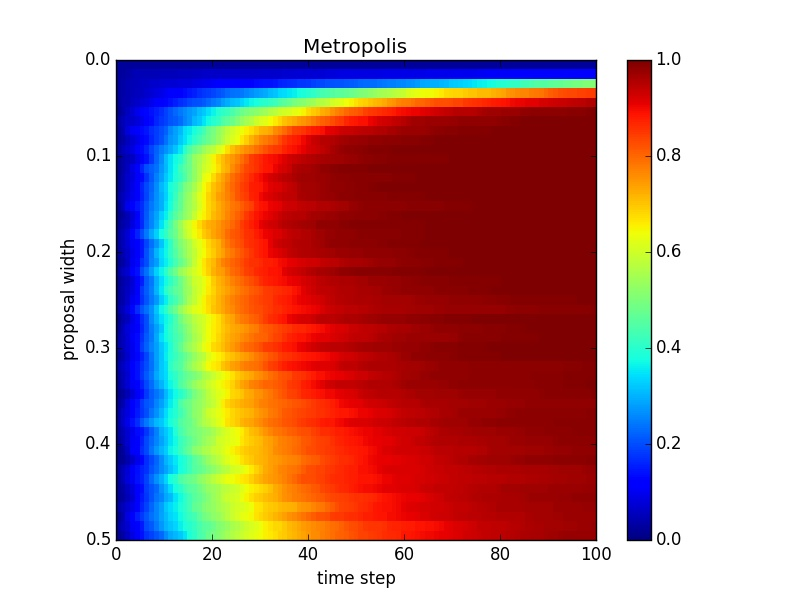
\includegraphics[width=\linewidth]{UQPlot_ConvWidth_Gaussian_001D_00_AdaF.jpg}
\endminipage\hfill
\minipage{0.5\textwidth}
	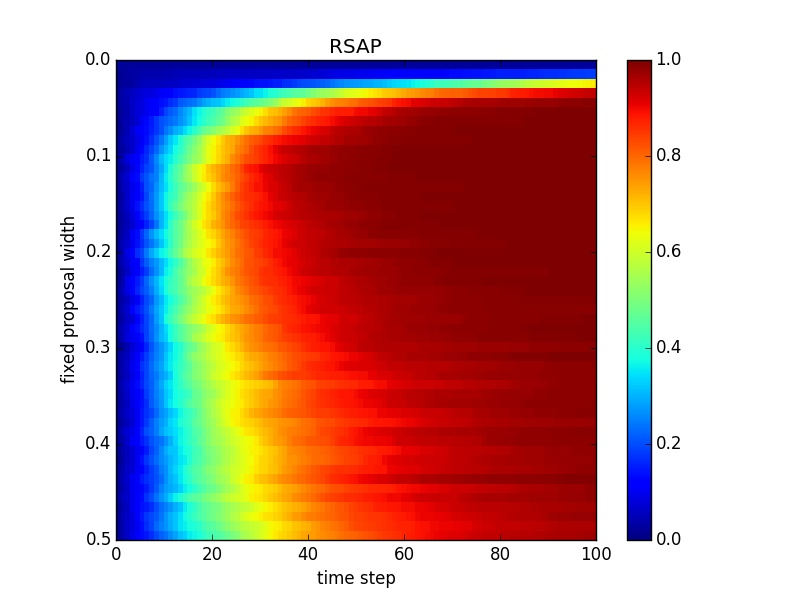
\includegraphics[width=\linewidth]{UQPlot_ConvWidth_Gaussian_001D_00_AdaT.jpg}
\endminipage\hfill
\caption{Plots of the cumulative convergence of Metropolis (left) and RSAP (right) on a 1D Gaussian. 100 steps per chain, 500 chains per width value, threshold of 0.003.}
\end{figure}

\begin{figure}[!htb]
\minipage{0.5\textwidth}
	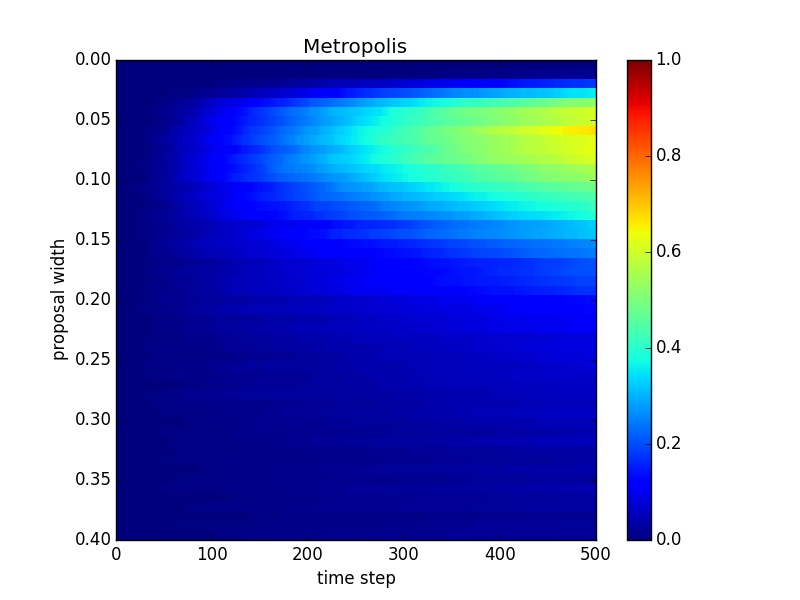
\includegraphics[width=\linewidth]{UQPlot_ConvWidth_Gaussian_003D_00_AdaF.jpg}
\endminipage\hfill
\minipage{0.5\textwidth}
	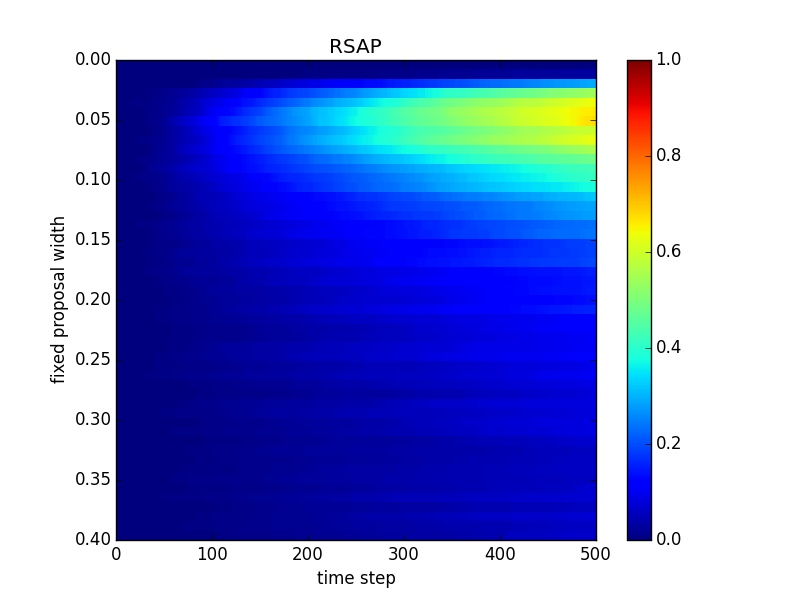
\includegraphics[width=\linewidth]{UQPlot_ConvWidth_Gaussian_003D_00_AdaT.jpg}
\endminipage\hfill
\caption{Plots of the cumulative convergence of Metropolis (left) and RSAP (right) on a 3D Gaussian. 500 steps per chain, 1000 chains per width value, threshold of 0.003. Note the different vertical axis scale.}
\end{figure}

\begin{figure}[!htb]
\minipage{0.5\textwidth}
	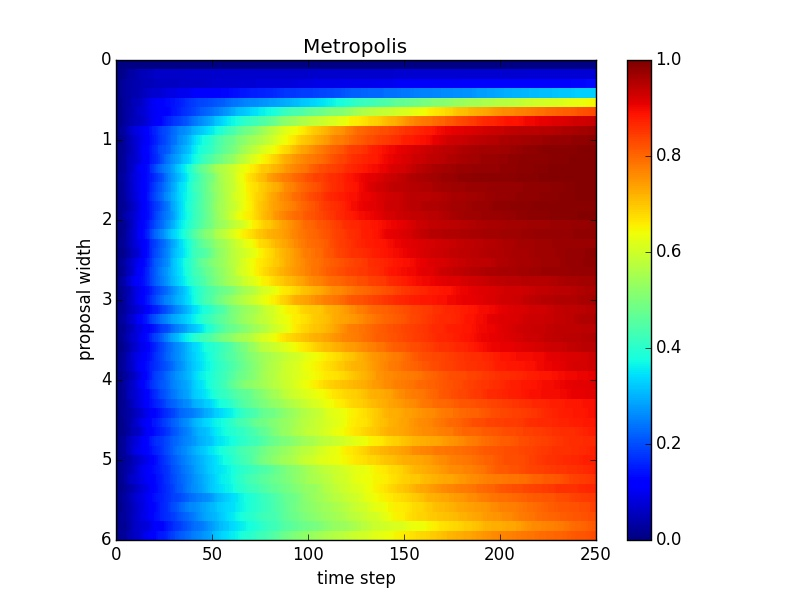
\includegraphics[width=\linewidth]{UQPlot_ConvWidth_Ackley_001D_00_AdaF.jpg}
\endminipage\hfill
\minipage{0.5\textwidth}
	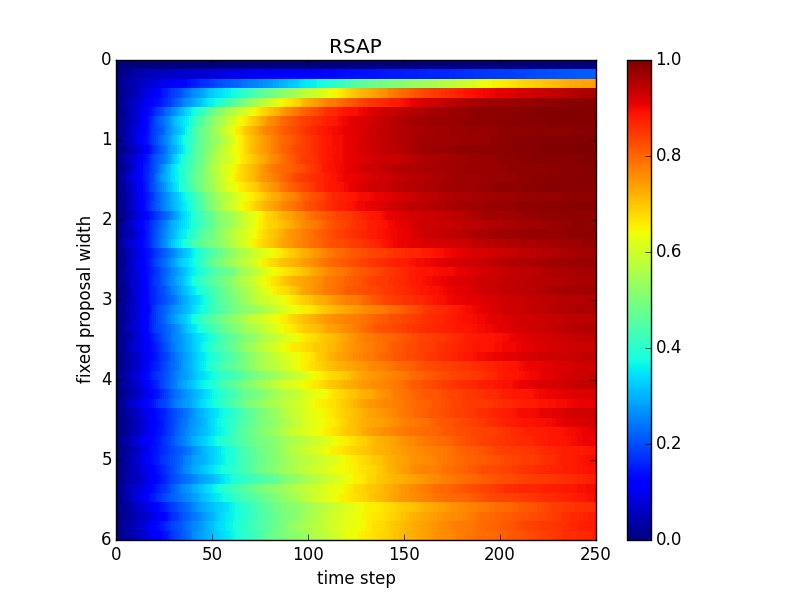
\includegraphics[width=\linewidth]{UQPlot_ConvWidth_Ackley_001D_00_AdaT.jpg}
\endminipage\hfill
\caption{Plots of the cumulative convergence of Metropolis (left) and RSAP (right) on a 1D Ackley function. 150 steps per chain, 1000 chains per width value, threshold of 0.8.}
\end{figure}

\begin{figure}[!htb]
\minipage{0.5\textwidth}
	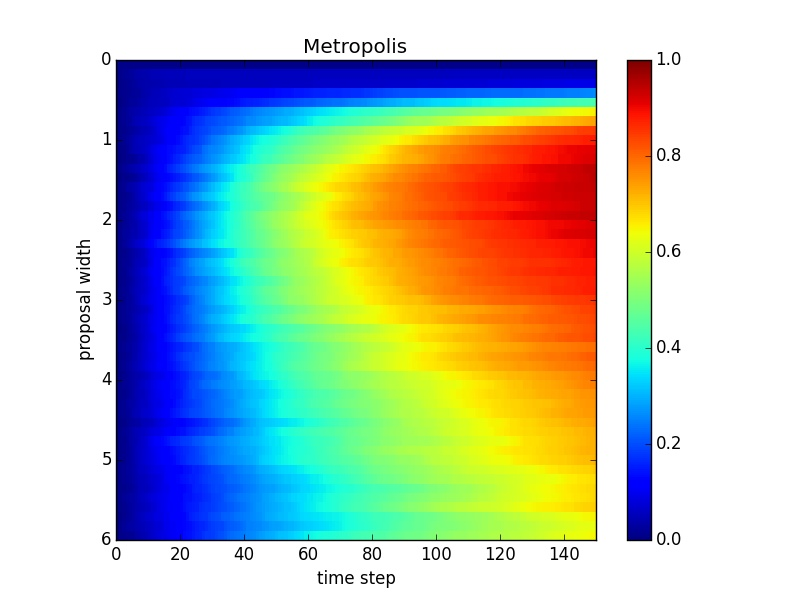
\includegraphics[width=\linewidth]{UQPlot_ConvWidth_Ackley_001D_01_AdaF.jpg}
\endminipage\hfill
\minipage{0.5\textwidth}
	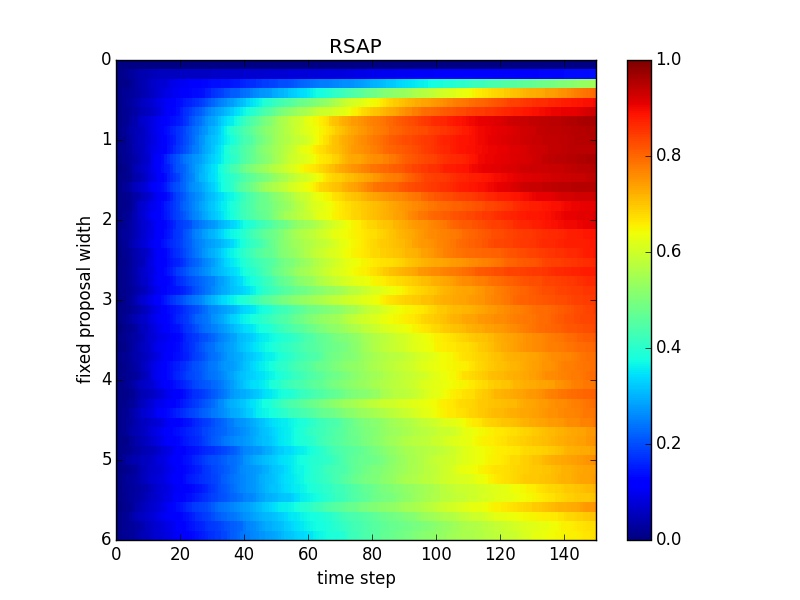
\includegraphics[width=\linewidth]{UQPlot_ConvWidth_Ackley_001D_01_AdaT.jpg}
\endminipage\hfill
\caption{Plots of the cumulative convergence of Metropolis (left) and RSAP (right) on a 1D Ackley function. 150 steps per chain, 1000 chains per width value, threshold of 0.8.}
\end{figure}

\begin{figure}[!htb]
\minipage{0.5\textwidth}
	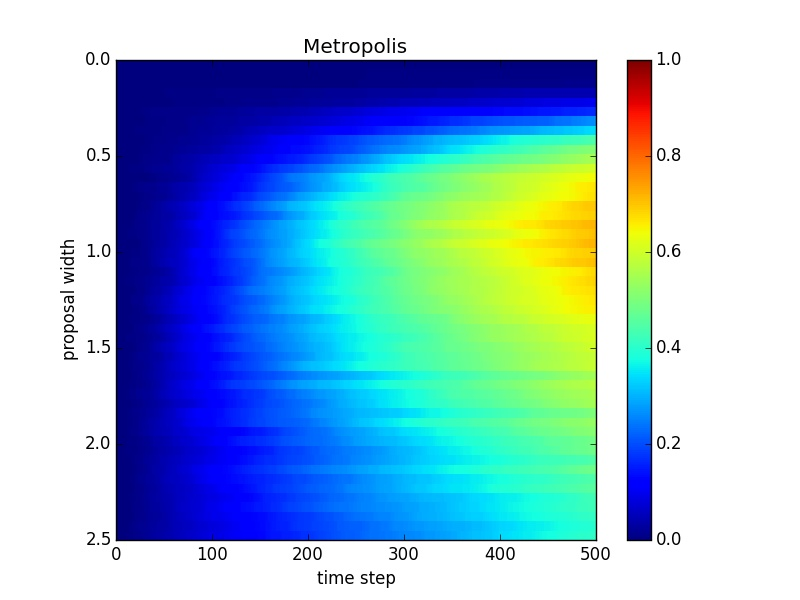
\includegraphics[width=\linewidth]{UQPlot_ConvWidth_Ackley_002D_00_AdaF.jpg}
\endminipage\hfill
\minipage{0.5\textwidth}
	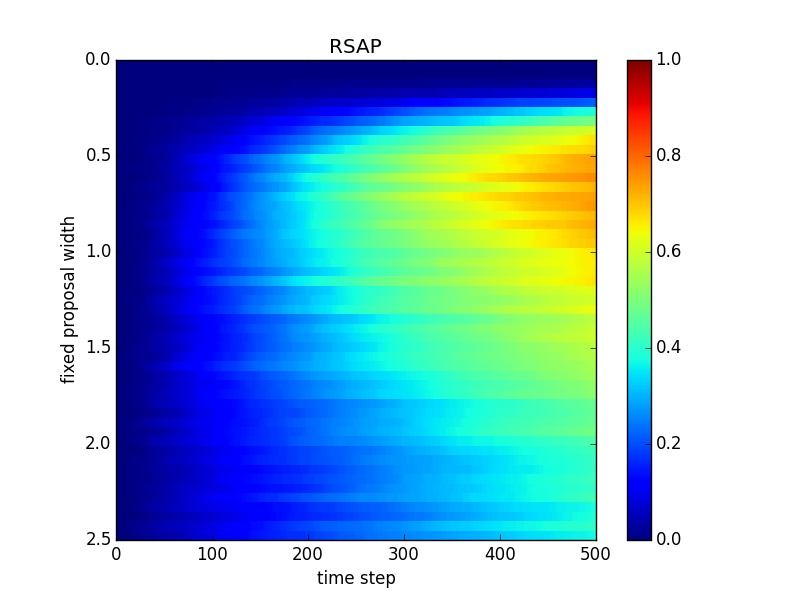
\includegraphics[width=\linewidth]{UQPlot_ConvWidth_Ackley_002D_00_AdaT.jpg}
\endminipage\hfill
\caption{Plots of the cumulative convergence of Metropolis (left) and RSAP (right) on a 2D Ackley function. 500 steps per chain, 1000 chains per width value, threshold of 0.8, $\Delta_0 = 3.5$.}
\end{figure}

\begin{figure}[!htb]
\minipage{0.5\textwidth}
	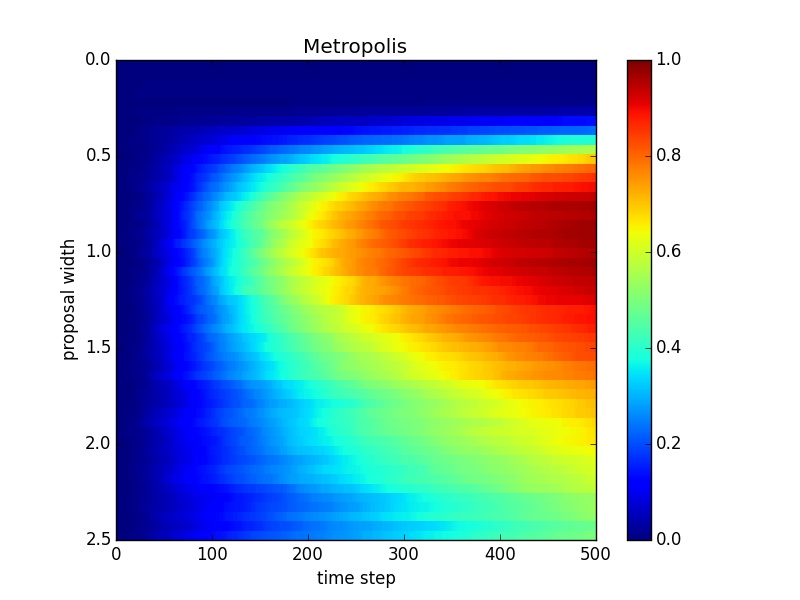
\includegraphics[width=\linewidth]{UQPlot_ConvWidth_Ackley_002D_01_AdaF.jpg}
\endminipage\hfill
\minipage{0.5\textwidth}
	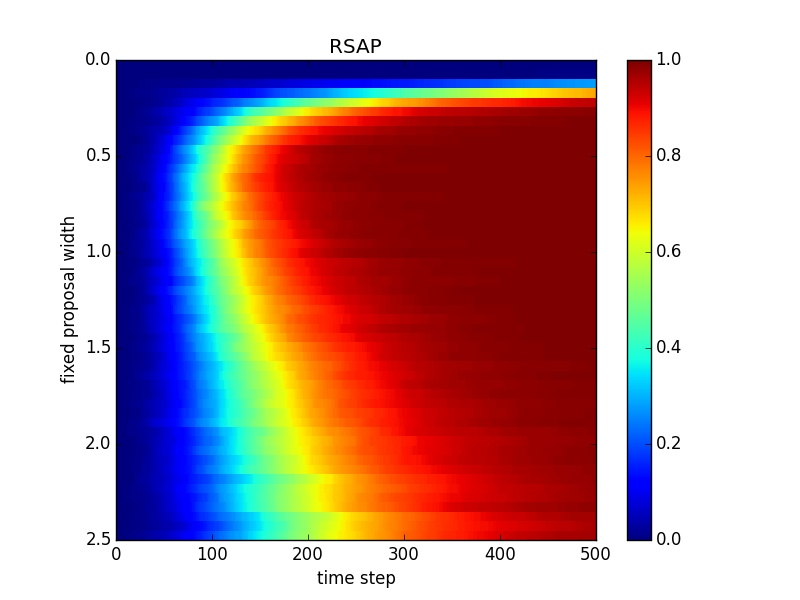
\includegraphics[width=\linewidth]{UQPlot_ConvWidth_Ackley_002D_01_AdaT.jpg}
\endminipage\hfill
\caption{Plots of the cumulative convergence of Metropolis (left) and RSAP (right) on a 2D Ackley function. 500 steps per chain, 1000 chains per width value, threshold of 0.8, $\Delta_0 = 0.5$.}
\end{figure}

\begin{figure}[!htb]
\minipage{0.5\textwidth}
	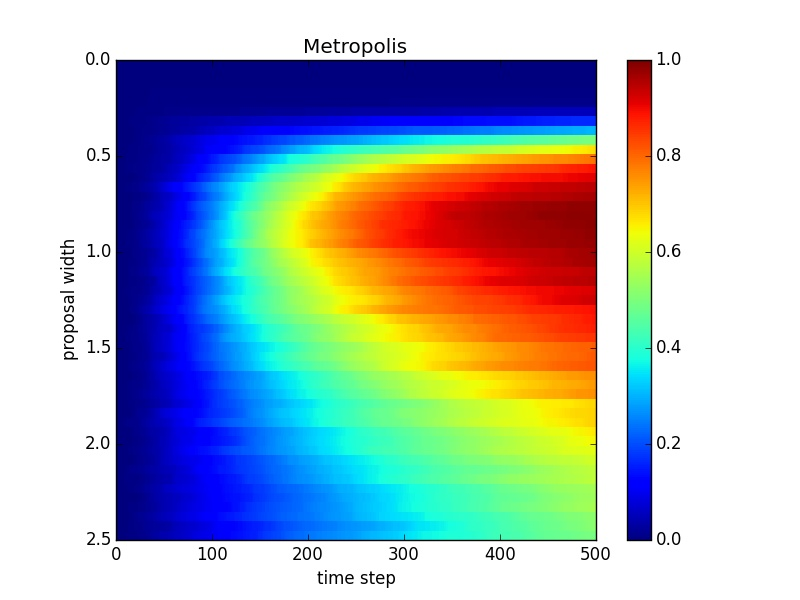
\includegraphics[width=\linewidth]{UQPlot_ConvWidth_Ackley_002D_02_AdaF.jpg}
\endminipage\hfill
\minipage{0.5\textwidth}
	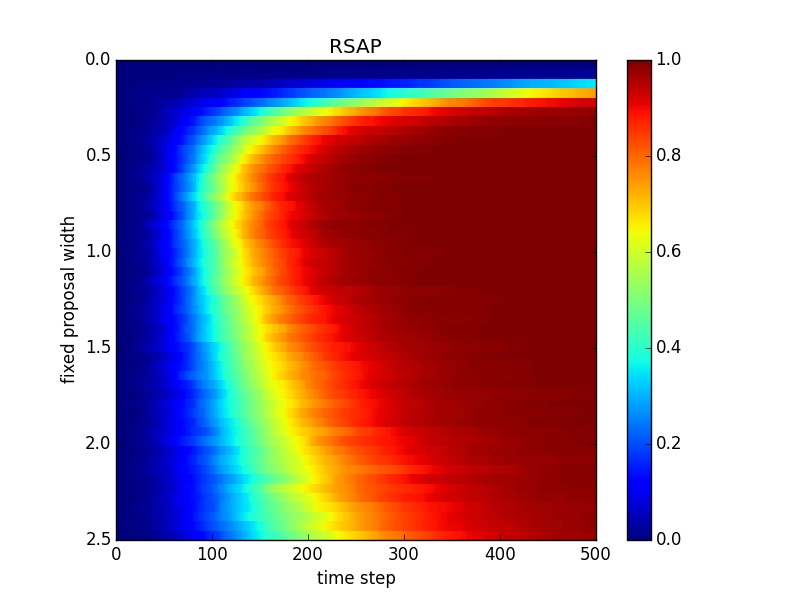
\includegraphics[width=\linewidth]{UQPlot_ConvWidth_Ackley_002D_02_AdaT.jpg}
\endminipage\hfill
\caption{Plots of the cumulative convergence of Metropolis (left) and RSAP (right) on a 2D Ackley function. 500 steps per chain, 1000 chains per width value, threshold of 0.8, $\Delta_0 = 0.01$.}
\end{figure}


\begin{comment}
Use this as impetus for convergence vs. width graphs:

From Haario AP:
"It is well known that when the proposal distribution is too large, too many candidate points are rejected and therefore the chain covers slowly the target distribution. On the other hand, when the proposal distribution is too small, too many candidate points are accepted and the chain converges slowly again. In addition, to ensure computational effciency one should choose the proposal distribution so that sampling from it would be fast and easy."
\end{comment}


\section{Application: galaxy merger simulation}



\section{Conclusions}




%%%%%%%%%%%%%%%
%%%%%%%%%%%%%%%
%%%%% THE END %%%%%
%%%%%%%%%%%%%%%
%%%%%%%%%%%%%%%

\section*{Acknowledgments}
We would like to acknowledge the assistance of volunteers in putting
together this example manuscript and supplement.

\bibliographystyle{siamplain}
\bibliography{references}

\begin{thebibliography}{10}

\bibitem{RWM} Sherlock, Chris; Fearnhead, Paul; Roberts, Gareth O. "The Random Walk Metropolis: Linking Theory and Practice Through a Case Study." \textit{Statist. Sci.} 25 (2010), no. 2, 172-190. doi:10.1214/10-STS327. https://projecteuclid.org/euclid.ss/1290175840

\bibitem{Hastings} Hastings, W. K. 1970. "Monte Carlo sampling methods using Markov chains and their applications." \textit{Biometrika}, 57:97-109.

\bibitem{Metro} Metropolis, N., Rosenbluth, A. W., Rosenbluth, M. N., Teller, A. H., and Teller, E. 1953. "Equation of state calculations by fast computing machines." \textit{Journal of Chemical Physics}, 21:1087-1092.

\bibitem{GelmanBayes} Gelman, A., Carlin, J., Stern, H., Dunson, D., Vehtari, A., and Rubin, D. \textit{Bayesian Data Analysis}, 3e. 2014. CRC Press.

\bibitem{HaarioAP} H. Haario, E. Saksman, and J. Tamminen (1999). Adaptive proposal distribution for random walk Metropolis algorithm. Comput. Stat. 14 375-395.

\bibitem{HaarioAM} Harrio, H., Saksman, E., Tamminen, J. "An Adaptive Metropolis Algorithm." \textit{Bernoulli} 7(2), 2001, 223-242.

\bibitem{AdaptReview} Gareth O. Roberts and Jeffrey S. Rosenthal (2012) Examples of Adaptive MCMC, Journal of Computational and Graphical Statistics, 18:2, 349-367, DOI: 10.1198/jcgs.2009.06134

\bibitem{RRAdaptErgo} Gareth O. Roberts and Jeffrey S. Rosenthal. "Coupling and Ergodicity of Adaptive Markov Chain Monte Carlo Algorithms." \textit{Journal of Applied Probability}, Vol. 44, No. 2 (Jun., 2007), pp. 458-475

\bibitem{Interact} Liu Jing, Prahlad Vadakkepat. "Interacting MCMC particle filter for tracking maneuvering target." \textit{Digital Signal Processing.} Volume 20, Issue 2, 2010, Pages 561-574.

% Harrio adaptive RWM Comput Stat
% https://link.springer.com/article/10.1007/s001800050022

% file:///D:/Graham/Documents/MTSU_HDD/Research/ApCN%20MCMC.pdf
% file:///D:/Graham/Documents/MTSU_HDD/Research/Handbook%20of%20MCMC.pdf
% 
% 
% 

\bibitem{citizen} A. Holincheck, J. Wallin, K. Borne, L. Fortson, C. Lintott, A M. Smith, S. Bamford, W. Keel, and M. Parrish, ``Galaxy Zoo: Mergers - Dynamical Models of Interacting Galaxies.'' \textit{MNRAS}, (2016). Vol. 459, Is. 1, 720-745.

\bibitem{galaxyFE} H. Mo, F. Bosch, and S. White, \textit{Galaxy Formation and Evolution}, 2010, Cambridge University Press.

\bibitem{jspam} J. Wallin, A. Holincheck, and A. Harvey, ``JSPAM: A restricted three-body code for simulating interacting galaxies.'' \textit{Astronomy and Computing} 16, (2016). 26-33.

\end{thebibliography}

\end{document}
